\section{Supplemental to Chapter~\ref{ch:pmao}}
%\label{sec:result_balibase}

% Table generated by Excel2LaTeX from sheet 'pasta varaints (2)'
\begin{table}[!htbp]
	\centering
	\small
	\caption{FN rate achieved by the four variants of PASTA for each dataset in set A. On each row, the lower (better) FN rate values are marked with darker color.}
	\begin{tabular}{|l|r|r|r|r|}
		\hline
		\multirow{2}{*}{Dataset} & \multicolumn{4}{c|}{FN rate of PASTA variants } \\
		\cline{2-5}          & \multicolumn{1}{l|}{PASTA-3I-D} & \multicolumn{1}{l|}{PASTA-8I-D} & \multicolumn{1}{l|}{PASTA-3I-S} & \multicolumn{1}{l|}{PASTA-8I-S} \\
		\hline
		BB11005 & \cellcolor[rgb]{ .384,  .745,  .478}0.27 & \cellcolor[rgb]{ .988,  1,  .992}0.55 & \cellcolor[rgb]{ .584,  .827,  .647}0.36 & \cellcolor[rgb]{ .384,  .745,  .478}0.27 \\
		\hline
		BB11018 & \cellcolor[rgb]{ .384,  .745,  .478}0.27 & \cellcolor[rgb]{ .384,  .745,  .478}0.27 & \cellcolor[rgb]{ .584,  .827,  .647}0.36 & \cellcolor[rgb]{ .988,  1,  .992}0.55 \\
		\hline
		BB11020 & \cellcolor[rgb]{ .686,  .871,  .733}0.67 & \cellcolor[rgb]{ .988,  1,  .992}0.83 & \cellcolor[rgb]{ .384,  .745,  .478}0.50 & \cellcolor[rgb]{ .384,  .745,  .478}0.50 \\
		\hline
		BB11033 & \cellcolor[rgb]{ .502,  .796,  .58}0.50 & \cellcolor[rgb]{ .384,  .745,  .478}0.38 & \cellcolor[rgb]{ .624,  .847,  .682}0.63 & \cellcolor[rgb]{ .988,  1,  .992}1.00 \\
		\hline
		BB12001 & \cellcolor[rgb]{ .988,  1,  .992}0.50 & \cellcolor[rgb]{ .384,  .745,  .478}0.25 & \cellcolor[rgb]{ .686,  .871,  .733}0.38 & \cellcolor[rgb]{ .686,  .871,  .733}0.38 \\
		\hline
		BB12013 & \cellcolor[rgb]{ .988,  1,  .992}0.20 & \cellcolor[rgb]{ .988,  1,  .992}0.20 & \cellcolor[rgb]{ .988,  1,  .992}0.20 & \cellcolor[rgb]{ .988,  1,  .992}0.20 \\
		\hline
		BB12022 & \cellcolor[rgb]{ .384,  .745,  .478}0.00 & \cellcolor[rgb]{ .384,  .745,  .478}0.00 & \cellcolor[rgb]{ .384,  .745,  .478}0.00 & \cellcolor[rgb]{ .988,  1,  .992}0.50 \\
		\hline
		BB12035 & \cellcolor[rgb]{ .467,  .78,  .549}0.04 & \cellcolor[rgb]{ .384,  .745,  .478}0.00 & \cellcolor[rgb]{ .467,  .78,  .549}0.04 & \cellcolor[rgb]{ .988,  1,  .992}0.29 \\
		\hline
		BB12044 & \cellcolor[rgb]{ .988,  1,  .992}0.50 & \cellcolor[rgb]{ .988,  1,  .992}0.50 & \cellcolor[rgb]{ .384,  .745,  .478}0.38 & \cellcolor[rgb]{ .384,  .745,  .478}0.38 \\
		\hline
		BB20002 & \cellcolor[rgb]{ .988,  1,  .992}0.65 & \cellcolor[rgb]{ .988,  1,  .992}0.65 & \cellcolor[rgb]{ .988,  1,  .992}0.65 & \cellcolor[rgb]{ .988,  1,  .992}0.65 \\
		\hline
		BB20010 & \cellcolor[rgb]{ .988,  1,  .992}0.38 & \cellcolor[rgb]{ .835,  .933,  .863}0.35 & \cellcolor[rgb]{ .686,  .871,  .733}0.31 & \cellcolor[rgb]{ .384,  .745,  .478}0.23 \\
		\hline
		BB20022 & \cellcolor[rgb]{ .988,  1,  .992}0.11 & \cellcolor[rgb]{ .988,  1,  .992}0.11 & \cellcolor[rgb]{ .988,  1,  .992}0.11 & \cellcolor[rgb]{ .988,  1,  .992}0.11 \\
		\hline
		BB20033 & \cellcolor[rgb]{ .988,  1,  .992}0.38 & \cellcolor[rgb]{ .835,  .933,  .863}0.36 & \cellcolor[rgb]{ .988,  1,  .992}0.38 & \cellcolor[rgb]{ .384,  .745,  .478}0.29 \\
		\hline
		BB20041 & \cellcolor[rgb]{ .502,  .792,  .58}0.40 & \cellcolor[rgb]{ .384,  .745,  .478}0.38 & \cellcolor[rgb]{ .624,  .843,  .682}0.42 & \cellcolor[rgb]{ .988,  1,  .992}0.49 \\
		\hline
		BB30002 & \cellcolor[rgb]{ .988,  1,  .992}0.32 & \cellcolor[rgb]{ .988,  1,  .992}0.32 & \cellcolor[rgb]{ .988,  1,  .992}0.32 & \cellcolor[rgb]{ .988,  1,  .992}0.32 \\
		\hline
		BB30008 & \cellcolor[rgb]{ .384,  .745,  .478}0.33 & \cellcolor[rgb]{ .384,  .745,  .478}0.33 & \cellcolor[rgb]{ .584,  .827,  .647}0.36 & \cellcolor[rgb]{ .988,  1,  .992}0.42 \\
		\hline
		BB30015 & \cellcolor[rgb]{ .384,  .745,  .478}0.17 & \cellcolor[rgb]{ .384,  .745,  .478}0.17 & \cellcolor[rgb]{ .384,  .745,  .478}0.17 & \cellcolor[rgb]{ .988,  1,  .992}0.33 \\
		\hline
		BB30022 & \cellcolor[rgb]{ .988,  1,  .992}0.54 & \cellcolor[rgb]{ .584,  .827,  .647}0.51 & \cellcolor[rgb]{ .384,  .745,  .478}0.49 & \cellcolor[rgb]{ .584,  .827,  .647}0.51 \\
		\hline
		BB40001 & \cellcolor[rgb]{ .988,  1,  .992}0.68 & \cellcolor[rgb]{ .384,  .745,  .478}0.48 & \cellcolor[rgb]{ .624,  .847,  .682}0.56 & \cellcolor[rgb]{ .384,  .745,  .478}0.48 \\
		\hline
		BB40013 & \cellcolor[rgb]{ .384,  .745,  .478}0.38 & \cellcolor[rgb]{ .384,  .745,  .478}0.38 & \cellcolor[rgb]{ .384,  .745,  .478}0.38 & \cellcolor[rgb]{ .988,  1,  .992}0.47 \\
		\hline
		BB40025 & \cellcolor[rgb]{ .384,  .745,  .478}0.00 & \cellcolor[rgb]{ .384,  .745,  .478}0.00 & \cellcolor[rgb]{ .384,  .745,  .478}0.00 & \cellcolor[rgb]{ .988,  1,  .992}0.09 \\
		\hline
		BB40038 & \cellcolor[rgb]{ .988,  1,  .992}0.25 & \cellcolor[rgb]{ .988,  1,  .992}0.25 & \cellcolor[rgb]{ .988,  1,  .992}0.25 & \cellcolor[rgb]{ .988,  1,  .992}0.25 \\
		\hline
		BB40048 & \cellcolor[rgb]{ .384,  .745,  .478}0.29 & \cellcolor[rgb]{ .988,  1,  .992}0.43 & \cellcolor[rgb]{ .384,  .745,  .478}0.29 & \cellcolor[rgb]{ .384,  .745,  .478}0.29 \\
		\hline
		BB50001 & \cellcolor[rgb]{ .988,  1,  .992}0.32 & \cellcolor[rgb]{ .384,  .745,  .478}0.29 & \cellcolor[rgb]{ .988,  1,  .992}0.32 & \cellcolor[rgb]{ .384,  .745,  .478}0.29 \\
		\hline
		BB50005 & \cellcolor[rgb]{ .988,  1,  .992}0.38 & \cellcolor[rgb]{ .988,  1,  .992}0.38 & \cellcolor[rgb]{ .988,  1,  .992}0.38 & \cellcolor[rgb]{ .988,  1,  .992}0.38 \\
		\hline
		BB50010 & \cellcolor[rgb]{ .988,  1,  .992}0.07 & \cellcolor[rgb]{ .384,  .745,  .478}0.00 & \cellcolor[rgb]{ .988,  1,  .992}0.07 & \cellcolor[rgb]{ .384,  .745,  .478}0.00 \\
		\hline
		BB50016 & \cellcolor[rgb]{ .384,  .745,  .478}0.27 & \cellcolor[rgb]{ .988,  1,  .992}0.47 & \cellcolor[rgb]{ .384,  .745,  .478}0.27 & \cellcolor[rgb]{ .384,  .745,  .478}0.27 \\
		\hline		
	\end{tabular}%
	\label{tab:pasta-variants-a}%
\end{table}%



\begin{table}[!htbp]
	\centering
	\small
	\caption{FN rate achieved by the four variants of PASTA for each dataset in set B. On each row, the lower (better) FN rate values are marked with darker color.}
	\begin{tabular}{|l|r|r|r|r|}
		\hline
		\multirow{2}{*}{Dataset} & \multicolumn{4}{c|}{FN rate of PASTA variants} \\
		\cline{2-5}          & \multicolumn{1}{l|}{PASTA-3I-D} & \multicolumn{1}{l|}{PASTA-8I-D} & \multicolumn{1}{l|}{PASTA-3I-S} & \multicolumn{1}{l|}{PASTA-8I-S} \\
		\hline
		BB11007 & \cellcolor[rgb]{ .988,  1,  .992}0.67 & \cellcolor[rgb]{ .384,  .745,  .478}0.50 & \cellcolor[rgb]{ .988,  1,  .992}0.67 & \cellcolor[rgb]{ .384,  .745,  .478}0.50 \\
		\hline
		BB11019 & \cellcolor[rgb]{ .988,  1,  .992}0.43 & \cellcolor[rgb]{ .682,  .871,  .733}0.29 & \cellcolor[rgb]{ .384,  .745,  .478}0.14 & \cellcolor[rgb]{ .682,  .871,  .733}0.29 \\
		\hline
		BB11034 & \cellcolor[rgb]{ .384,  .745,  .478}0.20 & \cellcolor[rgb]{ .686,  .871,  .733}0.40 & \cellcolor[rgb]{ .686,  .871,  .733}0.40 & \cellcolor[rgb]{ .988,  1,  .992}0.60 \\
		\hline
		BB11038 & \cellcolor[rgb]{ .384,  .745,  .478}0.40 & \cellcolor[rgb]{ .384,  .745,  .478}0.40 & \cellcolor[rgb]{ .988,  1,  .992}0.60 & \cellcolor[rgb]{ .988,  1,  .992}0.60 \\
		\hline
		BB12005 & \cellcolor[rgb]{ .384,  .745,  .478}0.33 & \cellcolor[rgb]{ .384,  .745,  .478}0.33 & \cellcolor[rgb]{ .384,  .745,  .478}0.33 & \cellcolor[rgb]{ .988,  1,  .992}0.50 \\
		\hline
		BB12026 & \cellcolor[rgb]{ .384,  .745,  .478}0.40 & \cellcolor[rgb]{ .624,  .843,  .682}0.53 & \cellcolor[rgb]{ .624,  .843,  .682}0.53 & \cellcolor[rgb]{ .988,  1,  .992}0.73 \\
		\hline
		BB12029 & \cellcolor[rgb]{ .988,  1,  .992}0.44 & \cellcolor[rgb]{ .988,  1,  .992}0.44 & \cellcolor[rgb]{ .988,  1,  .992}0.44 & \cellcolor[rgb]{ .988,  1,  .992}0.44 \\
		\hline
		BB12037 & \cellcolor[rgb]{ .482,  .784,  .561}0.30 & \cellcolor[rgb]{ .584,  .827,  .647}0.40 & \cellcolor[rgb]{ .988,  1,  .992}0.80 & \cellcolor[rgb]{ .384,  .745,  .478}0.20 \\
		\hline
		BB20002 & \cellcolor[rgb]{ .988,  1,  .992}0.65 & \cellcolor[rgb]{ .988,  1,  .992}0.65 & \cellcolor[rgb]{ .988,  1,  .992}0.65 & \cellcolor[rgb]{ .988,  1,  .992}0.65 \\
		\hline
		BB20012 & \cellcolor[rgb]{ .686,  .871,  .733}0.29 & \cellcolor[rgb]{ .686,  .871,  .733}0.29 & \cellcolor[rgb]{ .988,  1,  .992}0.33 & \cellcolor[rgb]{ .384,  .745,  .478}0.25 \\
		\hline
		BB20030 & \cellcolor[rgb]{ .384,  .745,  .478}0.64 & \cellcolor[rgb]{ .384,  .745,  .478}0.64 & \cellcolor[rgb]{ .502,  .792,  .58}0.66 & \cellcolor[rgb]{ .988,  1,  .992}0.75 \\
		\hline
		BB20037 & \cellcolor[rgb]{ .988,  1,  .992}0.29 & \cellcolor[rgb]{ .384,  .745,  .478}0.13 & \cellcolor[rgb]{ .867,  .949,  .886}0.26 & \cellcolor[rgb]{ .804,  .922,  .835}0.24 \\
		\hline
		BB30003 & \cellcolor[rgb]{ .682,  .871,  .733}0.30 & \cellcolor[rgb]{ .682,  .871,  .733}0.30 & \cellcolor[rgb]{ .988,  1,  .992}0.31 & \cellcolor[rgb]{ .384,  .745,  .478}0.29 \\
		\hline
		BB30011 & \cellcolor[rgb]{ .988,  1,  .992}0.35 & \cellcolor[rgb]{ .988,  1,  .992}0.35 & \cellcolor[rgb]{ .988,  1,  .992}0.35 & \cellcolor[rgb]{ .988,  1,  .992}0.35 \\
		\hline
		BB30021 & \cellcolor[rgb]{ .522,  .804,  .596}0.38 & \cellcolor[rgb]{ .451,  .773,  .537}0.36 & \cellcolor[rgb]{ .988,  1,  .992}0.53 & \cellcolor[rgb]{ .384,  .745,  .478}0.34 \\
		\hline
		BB30026 & \cellcolor[rgb]{ .988,  1,  .992}0.22 & \cellcolor[rgb]{ .384,  .745,  .478}0.19 & \cellcolor[rgb]{ .988,  1,  .992}0.22 & \cellcolor[rgb]{ .682,  .871,  .733}0.21 \\
		\hline
		BB40006 & \cellcolor[rgb]{ .988,  1,  .992}0.00 & \cellcolor[rgb]{ .988,  1,  .992}0.00 & \cellcolor[rgb]{ .988,  1,  .992}0.00 & \cellcolor[rgb]{ .988,  1,  .992}0.00 \\
		\hline
		BB40009 & \cellcolor[rgb]{ .988,  1,  .992}0.19 & \cellcolor[rgb]{ .988,  1,  .992}0.19 & \cellcolor[rgb]{ .988,  1,  .992}0.19 & \cellcolor[rgb]{ .988,  1,  .992}0.19 \\
		\hline
		BB40019 & \cellcolor[rgb]{ .988,  1,  .992}0.43 & \cellcolor[rgb]{ .988,  1,  .992}0.43 & \cellcolor[rgb]{ .988,  1,  .992}0.43 & \cellcolor[rgb]{ .988,  1,  .992}0.43 \\
		\hline
		BB40033 & \cellcolor[rgb]{ .384,  .745,  .478}0.06 & \cellcolor[rgb]{ .988,  1,  .992}0.13 & \cellcolor[rgb]{ .988,  1,  .992}0.13 & \cellcolor[rgb]{ .988,  1,  .992}0.13 \\
		\hline
		BB50002 & \cellcolor[rgb]{ .988,  1,  .992}0.60 & \cellcolor[rgb]{ .384,  .745,  .478}0.50 & \cellcolor[rgb]{ .988,  1,  .992}0.60 & \cellcolor[rgb]{ .384,  .745,  .478}0.50 \\
		\hline
		BB50006 & \cellcolor[rgb]{ .384,  .745,  .478}0.21 & \cellcolor[rgb]{ .384,  .745,  .478}0.21 & \cellcolor[rgb]{ .835,  .933,  .863}0.26 & \cellcolor[rgb]{ .988,  1,  .992}0.28 \\
		\hline
		BB50009 & \cellcolor[rgb]{ .384,  .745,  .478}0.16 & \cellcolor[rgb]{ .784,  .914,  .82}0.24 & \cellcolor[rgb]{ .584,  .827,  .647}0.20 & \cellcolor[rgb]{ .988,  1,  .992}0.28 \\
		\hline
		BB50014 & \cellcolor[rgb]{ .988,  1,  .992}0.44 & \cellcolor[rgb]{ .384,  .745,  .478}0.41 & \cellcolor[rgb]{ .988,  1,  .992}0.44 & \cellcolor[rgb]{ .988,  1,  .992}0.44 \\
		\hline
	\end{tabular}%
	\label{tab:pasta-variants-b}%
\end{table}%

% Table generated by Excel2LaTeX from sheet 'stat test'
\begin{table}[!htbp]
	\small
	\centering
	\caption[Friedman test and Holm's post-hoc procedure to assess the significance of difference among the PASTA variants.]{\underline{Friedman Aligned Ranks test (Column 2):} Friedman Aligned ranks (lower is better) of the four variants of PASTA based on Table~\ref{tab:pasta-variants-a}, \ref{tab:pasta-variants-b}. We also show the computed statistics and corresponding $ p $-value. 
		\underline{Holm's post-hoc procedure (Columns 3 - 6):} Comparison among the PASTA variants using the Holm's post-hoc procedures. Each entry shows the adjusted $p$-value which indicates the significance of the difference in performance between two methods.}
	\begin{tabular}{|l|r||c|c|c|c|}
		\hline
		\multicolumn{1}{|c|}{1} & \multicolumn{1}{c||}{2} & \multicolumn{1}{c|}{3} & \multicolumn{1}{c|}{4} & \multicolumn{1}{c|}{5} & 6 \\
		\hline
		\multirow{2}{*}{\makecell{PASTA\\ variants}} & \multirow{2}{*}{\makecell{Friedman Aligned\\ rank*}} & \multicolumn{4}{c|}{Holm's adjusted $p$-value} \\
		\cline{3-6}          &       & 8I-D & 3I-D & 3I-S & 8I-S \\
		\hline
		8I-D  & 89.2843 & \multicolumn{1}{c|}{-} & \multicolumn{1}{r|}{1.0000} & \multicolumn{1}{r|}{0.4481} & \multicolumn{1}{r|}{0.1746} \\
		\hline
		3I-D  & 96.7941 & \multicolumn{1}{r|}{1.0000} & \multicolumn{1}{c|}{-} & \multicolumn{1}{r|}{0.8743} & \multicolumn{1}{r|}{0.4945} \\
		\hline
		3I-S  & 109.1275 & \multicolumn{1}{r|}{0.4481} & \multicolumn{1}{r|}{0.8743} & \multicolumn{1}{c|}{-} & \multicolumn{1}{r|}{1.0000} \\
		\hline
		8I-S  & 114.7941 & \multicolumn{1}{r|}{0.1746} & \multicolumn{1}{r|}{0.4945} & \multicolumn{1}{r|}{1.0000} & - \\
		\hline
		*Statistic & 4.8016 & \multicolumn{4}{c|}{\multirow{2}{*}{N/A}} \\
		\cline{1-2}    *$p$-value & 0.1869 & \multicolumn{4}{c|}{} \\
		\hline
	\end{tabular}%
	\label{tab:test-pasta-variants}%
\end{table}%

\begin{figure}[!htbp]%
	\begin{adjustwidth}{-1.0cm}{}
	\centering
	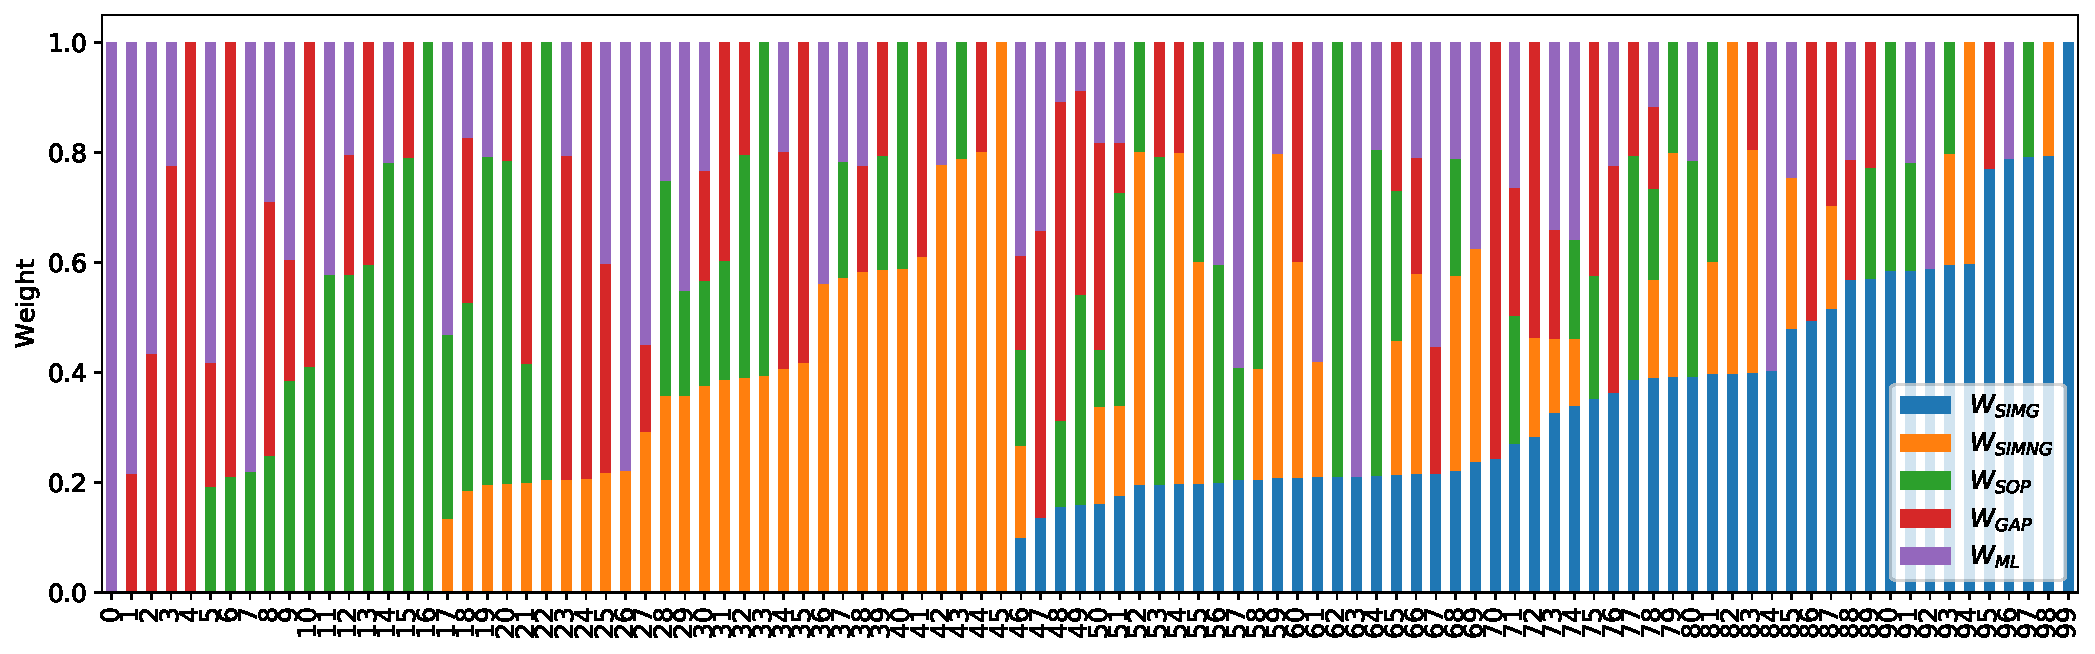
\includegraphics[width=\textwidth]{100-weights}
	\caption{100 well-spaced 5D weight vectors. Each vertical bar depicts one weight vector.}
	\label{fig:100-weights}
		\end{adjustwidth}
\end{figure}

% Table generated by Excel2LaTeX from sheet 'stat-8I-30w-S'
\begin{table}[htbp]
	\scriptsize
	\centering
	\caption{Comparison of the 100 solutions generated by PMAO using 100 input vectors with respect to PASTA's FN rate on set A datasets. For PMAO, we show the best FN rate along with the average FN rate 
		and count of its solutions better or equivalent to PASTA. The better values are marked with darker shade.}
	\begin{tabular}{|l|r|r|r||r|}
		\hline
		\multirow{2}{*}{Dataset} & \multirow{2}{*}{\makecell{PASTA\\FN rate}} & \multicolumn{3}{c|}{\makecell{PMAO solutions better \\or equivalent to PASTA}} \\
		\cline{3-5}          &       & \multicolumn{1}{l|}{Best FN} & \multicolumn{1}{l||}{Avg FN} & \multicolumn{1}{l|}{Count} \\
		\hline
		BB11005 & \cellcolor[rgb]{ .988,  1,  .992}0.55 & \cellcolor[rgb]{ .384,  .745,  .478}0.09 & \cellcolor[rgb]{ .71,  .882,  .757}0.34 & \cellcolor[rgb]{ .976,  .455,  .463}93 \\
		\hline
		BB11018 & \cellcolor[rgb]{ .988,  1,  .992}0.27 & \cellcolor[rgb]{ .384,  .745,  .478}0.18 & \cellcolor[rgb]{ .843,  .937,  .867}0.25 & \cellcolor[rgb]{ .988,  .855,  .867}25 \\
		\hline
		BB11033 & \cellcolor[rgb]{ .988,  1,  .992}0.38 & \cellcolor[rgb]{ .384,  .745,  .478}0.25 & \cellcolor[rgb]{ .957,  .984,  .965}0.37 & \cellcolor[rgb]{ .988,  .882,  .894}20 \\
		\hline
		BB11020 & \cellcolor[rgb]{ .988,  1,  .992}0.83 & \cellcolor[rgb]{ .384,  .745,  .478}0.17 & \cellcolor[rgb]{ .773,  .91,  .808}0.60 & \cellcolor[rgb]{ .973,  .412,  .42}100 \\
		\hline
		BB12001 & \cellcolor[rgb]{ .988,  1,  .992}0.25 & \cellcolor[rgb]{ .384,  .745,  .478}0.13 & \cellcolor[rgb]{ .933,  .976,  .945}0.24 & \cellcolor[rgb]{ .98,  .667,  .675}57 \\
		\hline
		BB12013 & \cellcolor[rgb]{ .988,  1,  .992}0.20 & \cellcolor[rgb]{ .384,  .745,  .478}0.00 & \cellcolor[rgb]{ .949,  .984,  .961}0.19 & \cellcolor[rgb]{ .976,  .42,  .427}99 \\
		\hline
		BB12022 & \cellcolor[rgb]{ .988,  1,  .992}0.00 & \cellcolor[rgb]{ .988,  1,  .992}0.00 & \cellcolor[rgb]{ .988,  1,  .992}0.00 & \cellcolor[rgb]{ .976,  .482,  .494}88 \\
		\hline
		BB12035 & \cellcolor[rgb]{ .988,  1,  .992}0.00 & \cellcolor[rgb]{ .988,  1,  .992}0.00 & \cellcolor[rgb]{ .988,  1,  .992}0.00 & \cellcolor[rgb]{ .988,  .988,  1}2 \\
		\hline
		BB12044 & \cellcolor[rgb]{ .988,  1,  .992}0.50 & \cellcolor[rgb]{ .384,  .745,  .478}0.25 & \cellcolor[rgb]{ .847,  .941,  .871}0.44 & \cellcolor[rgb]{ .973,  .412,  .42}100 \\
		\hline
		BB20001 & \cellcolor[rgb]{ .988,  1,  .992}0.54 & \cellcolor[rgb]{ .384,  .745,  .478}0.08 & \cellcolor[rgb]{ .886,  .957,  .906}0.46 & \cellcolor[rgb]{ .98,  .596,  .604}69 \\
		\hline
		BB20010 & \cellcolor[rgb]{ .988,  1,  .992}0.35 & \cellcolor[rgb]{ .384,  .745,  .478}0.08 & \cellcolor[rgb]{ .863,  .945,  .886}0.29 & \cellcolor[rgb]{ .976,  .502,  .51}85 \\
		\hline
		BB20022 & \cellcolor[rgb]{ .988,  1,  .992}0.11 & \cellcolor[rgb]{ .384,  .745,  .478}0.09 & \cellcolor[rgb]{ .969,  .992,  .976}0.11 & \cellcolor[rgb]{ .984,  .804,  .812}34 \\
		\hline
		BB20033 & \cellcolor[rgb]{ .988,  1,  .992}0.36 & \cellcolor[rgb]{ .384,  .745,  .478}0.27 & \cellcolor[rgb]{ .737,  .894,  .78}0.32 & \cellcolor[rgb]{ .984,  .82,  .831}31 \\
		\hline
		BB20041 & \cellcolor[rgb]{ .988,  1,  .992}0.38 & \cellcolor[rgb]{ .384,  .745,  .478}0.31 & \cellcolor[rgb]{ .839,  .937,  .867}0.36 & \cellcolor[rgb]{ .988,  .847,  .859}26 \\
		\hline
		BB30002 & \cellcolor[rgb]{ .988,  1,  .992}0.32 & \cellcolor[rgb]{ .384,  .745,  .478}0.14 & \cellcolor[rgb]{ .902,  .961,  .918}0.30 & \cellcolor[rgb]{ .98,  .694,  .706}52 \\
		\hline
		BB30008 & \cellcolor[rgb]{ .988,  1,  .992}0.33 & \cellcolor[rgb]{ .384,  .745,  .478}0.21 & \cellcolor[rgb]{ .859,  .945,  .882}0.31 & \cellcolor[rgb]{ .984,  .753,  .765}42 \\
		\hline
		BB30015 & \cellcolor[rgb]{ .988,  1,  .992}0.17 & \cellcolor[rgb]{ .384,  .745,  .478}0.11 & \cellcolor[rgb]{ .969,  .992,  .976}0.17 & \cellcolor[rgb]{ .984,  .788,  .8}36 \\
		\hline
		BB30022 & \cellcolor[rgb]{ .988,  1,  .992}0.51 & \cellcolor[rgb]{ .384,  .745,  .478}0.44 & \cellcolor[rgb]{ .91,  .965,  .925}0.50 & \cellcolor[rgb]{ .98,  .675,  .682}56 \\
		\hline
		BB40001 & \cellcolor[rgb]{ .988,  1,  .992}0.48 & \cellcolor[rgb]{ .384,  .745,  .478}0.32 & \cellcolor[rgb]{ .776,  .91,  .812}0.42 & \cellcolor[rgb]{ .988,  .878,  .89}21 \\
		\hline
		BB40013 & \cellcolor[rgb]{ .988,  1,  .992}0.38 & \cellcolor[rgb]{ .384,  .745,  .478}0.28 & \cellcolor[rgb]{ .765,  .906,  .8}0.34 & \cellcolor[rgb]{ .98,  .667,  .675}57 \\
		\hline
		BB40025 & \cellcolor[rgb]{ .988,  1,  .992}0.00 & \cellcolor[rgb]{ .988,  1,  .992}0.00 & \cellcolor[rgb]{ .988,  1,  .992}0.00 & \cellcolor[rgb]{ .98,  .643,  .651}61 \\
		\hline
		BB40038 & \cellcolor[rgb]{ .988,  1,  .992}0.25 & \cellcolor[rgb]{ .384,  .745,  .478}0.10 & \cellcolor[rgb]{ .769,  .906,  .808}0.20 & \cellcolor[rgb]{ .98,  .616,  .624}66 \\
		\hline
		BB40048 & \cellcolor[rgb]{ .988,  1,  .992}0.43 & \cellcolor[rgb]{ .384,  .745,  .478}0.29 & \cellcolor[rgb]{ .463,  .776,  .545}0.30 & \cellcolor[rgb]{ .973,  .412,  .42}100 \\
		\hline
		BB50001 & \cellcolor[rgb]{ .988,  1,  .992}0.29 & \cellcolor[rgb]{ .384,  .745,  .478}0.16 & \cellcolor[rgb]{ .902,  .961,  .918}0.27 & \cellcolor[rgb]{ .98,  .62,  .627}65 \\
		\hline
		BB50005 & \cellcolor[rgb]{ .988,  1,  .992}0.38 & \cellcolor[rgb]{ .384,  .745,  .478}0.13 & \cellcolor[rgb]{ .933,  .976,  .945}0.35 & \cellcolor[rgb]{ .973,  .412,  .42}100 \\
		\hline
		BB50010 & \cellcolor[rgb]{ .988,  1,  .992}0.00 & \cellcolor[rgb]{ .988,  1,  .992}0.00 & \cellcolor[rgb]{ .988,  1,  .992}0.00 & \cellcolor[rgb]{ .988,  .937,  .949}11 \\
		\hline
		BB50016 & \cellcolor[rgb]{ .988,  1,  .992}0.47 & \cellcolor[rgb]{ .384,  .745,  .478}0.07 & \cellcolor[rgb]{ .62,  .843,  .678}0.22 & \cellcolor[rgb]{ .976,  .42,  .427}99 \\
		\hline
	\end{tabular}%
	\label{tab:pmao-100}%
\end{table}%


\begin{figure}[!htbp]
	\begin{adjustwidth}{-1.2cm}{-1.2cm}
	\centering
	\def\names{{BB11005},{BB11018},{BB11033},{BB11020},{BB12001},{BB12013},{BB12022},{BB12035},{BB12044},{BB20001},{BB20010},{BB20022},{BB20033},{BB20041},{BB30002}, {BB30008}, {BB30015},{BB30022},{BB40001},{BB40013},{BB40025},{BB40038},{BB40048},{BB50001},{BB50005},{BB50010},{BB50016}}
	\foreach \name in \names {%
		\begin{subfigure}{0.22\textwidth} \includegraphics[width=\textwidth]{PMAO-A/\name-fn-ml} \caption{\name}\end{subfigure}
	}
	\end{adjustwidth}
	\caption{Visualization of PASTA output and the 30 solutions generated by PMAO for set A datasets. The x-axis and y-axis represent ML score and FN rate respectively.}
	\label{fig:ml-fn-a}
\end{figure}

\begin{figure}[!htbp]
	\begin{adjustwidth}{-1cm}{-1cm}
		\centering
		\def\names{{BB11007},{BB11034},{BB11038},{BB11019}, {BB12005},{BB12029},{BB12026},{BB12037}, {BB20002},{BB20012},{BB20030},{BB20037}, {BB30003},{BB30021},{BB30026},{BB30011},{BB40009},{BB40019},{BB40033},{BB40006},{BB50002},{BB50009},{BB50014},{BB50006}}
			\foreach \name in \names {%
			\begin{subfigure}{0.23\textwidth} \includegraphics[width=\textwidth]{PMAO-B/\name-fn-ml} \caption{\name}\end{subfigure}
		}
	\end{adjustwidth}
	\caption{Visualization of PASTA output and the 30 solutions generated by PMAO for set B datasets. The x-axis and y-axis represent ML score and FN rate respectively.}
	\label{fig:ml-fn-b}
\end{figure}

\begin{figure}[!htbp]
	\begin{adjustwidth}{-1.2cm}{-1.2cm}
		\centering
		\def\names{{BB11005},{BB11018},{BB11033},{BB11020},{BB12001},{BB12013},{BB12022},{BB12044},{BB20001},{BB20010},{BB20022},{BB20033},{BB20041},{BB30002}, {BB30008}, {BB30015},{BB30022},{BB40001},{BB40013},{BB40025},{BB40038},{BB40048},{BB50001},{BB50005},{BB50010},{BB50016}}
		\foreach \name in \names {%
		\begin{subfigure}{0.22\textwidth} \includegraphics[width=\textwidth]{weight-A/\name-good-weight} \caption{\name}\end{subfigure}
		}
	\end{adjustwidth}
	\caption{Visualization of weight vectors which lead PMAO to generate better or equivalent solutions to PASTA on datasets under set A. The y-axis portrays the weight values and the x-axis marks the achieved FN rate. The weight vectors are sorted in ascending order based on the achieved FN rate.}\label{fig:good-weight-a}
\end{figure}

\begin{figure}[!htbp]
	\begin{adjustwidth}{-1.2cm}{-1.2cm}
		\centering
		\def\names{{BB11007},{BB11034},{BB11038},{BB11019}, {BB12005},{BB12029},{BB12026},{BB12037}, {BB20002},{BB20012},{BB20030},{BB20037}, {BB30003},{BB30021},{BB30026},{BB30011},{BB40009},{BB40019},{BB40033},{BB40006},{BB50002},{BB50009},{BB50014},{BB50006}}
		\foreach \name in \names {%
			\begin{subfigure}{0.23\textwidth} \includegraphics[width=\textwidth]{weight-B/\name-good-weight} \caption{\name}\end{subfigure}
		}
	\caption{Visualization of weight vectors which lead PMAO to generate better or equivalent solutions to PASTA on datasets under set B. The y-axis portrays the weight values and the x-axis marks the achieved FN rate. The weight vectors are sorted in ascending order based on the achieved FN rate.}\label{fig:good-weight-b}
		\end{adjustwidth}
\end{figure}

\begin{figure}[!htbp]
	\begin{adjustwidth}{-1.2cm}{-1.2cm}
		\centering
		\def\names{{BB11007},{BB11034},{BB11038},{BB11019}, {BB12005},{BB12029},{BB12026},{BB12037}, {BB20002},{BB20012},{BB20030},{BB20037}, {BB30003},{BB30021},{BB30026},{BB30011},{BB40009},{BB40019},{BB40033},{BB40006},{BB50002},{BB50009},{BB50014},{BB50006}}
		\foreach \name in \names {%
		\begin{subfigure}{0.23\textwidth} \includegraphics[width=\textwidth]{weight-B-ml/\name-good-weight} \caption{\name}\end{subfigure}
	}

	\caption{Visualization of five weight vectors detected by machine learning approach on each datasets under set B. The y-axis portrays the weight values and the x-axis marks the achieved FN rate. The weight vectors are sorted in ascending order based on the achieved FN rate.}\label{fig:good-weight-ml}
		\end{adjustwidth}
\end{figure}



\begin{longtable}{|l|r|r|r||r|}
		%\centering
	\caption{Comparison of the 30 solutions generated by PMAO with respect to PASTA in terms of FN rate on on all BAliBASE 3.0 datasets. For PMAO, we show the best FN rate along with the average FN rate and count of its solutions better or equivalent to PASTA. The better values are marked with darker shade.} 	
	\label{tab:pmao-pasta-all} \\\hline
	\multirow{2}{*}{Dataset} & \multirow{2}{*}{\makecell{PASTA\\FN rate}} & \multicolumn{3}{c|}{\makecell{PMAO solutions better \\or equivalent to PASTA}} \\
	\cline{3-5}          &       & \multicolumn{1}{l|}{Best FN} & \multicolumn{1}{l||}{Avg FN} & \multicolumn{1}{l|}{Count} \\
	\hline
	\endfirsthead
	
	\multicolumn{3}{@{}l}{\ldots continued}\\\hline
	\multirow{2}{*}{Dataset} & \multirow{2}{*}{\makecell{PASTA\\FN rate}} & \multicolumn{3}{c|}{\makecell{PMAO solutions better \\or equivalent to PASTA}} \\
	\cline{3-5}          &       & \multicolumn{1}{l|}{Best FN} & \multicolumn{1}{l||}{Avg FN} & \multicolumn{1}{l|}{Count} \\
	\hline
	\endhead
	
	\hline
	\multicolumn{5}{r@{}}{continued \ldots}\\
	\endfoot
	\hline
	\endlastfoot
	
	BB11001 & \cellcolor[rgb]{ .988,  1,  .992}0.00 & \cellcolor[rgb]{ .988,  1,  .992}0.00 & \cellcolor[rgb]{ .988,  1,  .992}0.00 & \cellcolor[rgb]{ .973,  .412,  .42}30 \\
	\hline
	BB11002 & \cellcolor[rgb]{ .988,  1,  .992}0.40 & \cellcolor[rgb]{ .988,  1,  .992}0.40 & \cellcolor[rgb]{ .988,  1,  .992}0.40 & \cellcolor[rgb]{ .984,  .796,  .808}10 \\
	\hline
	BB11003 & \cellcolor[rgb]{ .988,  1,  .992}1.00 & \cellcolor[rgb]{ .384,  .745,  .478}0.00 & \cellcolor[rgb]{ .906,  .965,  .922}0.87 & \cellcolor[rgb]{ .973,  .412,  .42}30 \\
	\hline
	BB11004 & \cellcolor[rgb]{ .988,  1,  .992}0.00 & \cellcolor[rgb]{ .988,  1,  .992}0.00 & \cellcolor[rgb]{ .988,  1,  .992}0.00 & \cellcolor[rgb]{ .976,  .471,  .478}27 \\
	\hline
	BB11005 & \cellcolor[rgb]{ .988,  1,  .992}0.55 & \cellcolor[rgb]{ .384,  .745,  .478}0.09 & \cellcolor[rgb]{ .753,  .898,  .792}0.37 & \cellcolor[rgb]{ .976,  .451,  .459}28 \\
	\hline
	BB11006 & \cellcolor[rgb]{ .988,  1,  .992}0.40 & \cellcolor[rgb]{ .384,  .745,  .478}0.00 & \cellcolor[rgb]{ .647,  .855,  .702}0.18 & \cellcolor[rgb]{ .976,  .529,  .537}24 \\
	\hline
	BB11007 & \cellcolor[rgb]{ .988,  1,  .992}0.50 & \cellcolor[rgb]{ .384,  .745,  .478}0.33 & \cellcolor[rgb]{ .906,  .965,  .922}0.48 & \cellcolor[rgb]{ .98,  .702,  .71}15 \\
	\hline
	BB11008 & \cellcolor[rgb]{ .988,  1,  .992}1.00 & \cellcolor[rgb]{ .384,  .745,  .478}0.00 & \cellcolor[rgb]{ .706,  .878,  .749}0.53 & \cellcolor[rgb]{ .973,  .412,  .42}30 \\
	\hline
	BB11009 & \cellcolor[rgb]{ .988,  1,  .992}0.00 & \cellcolor[rgb]{ .988,  1,  .992}0.00 & \cellcolor[rgb]{ .988,  1,  .992}0.00 & \cellcolor[rgb]{ .976,  .451,  .459}28 \\
	\hline
	BB11010 & \cellcolor[rgb]{ .988,  1,  .992}0.00 & \cellcolor[rgb]{ .988,  1,  .992}0.00 & \cellcolor[rgb]{ .988,  1,  .992}0.00 & \cellcolor[rgb]{ .976,  .431,  .439}29 \\
	\hline
	BB11011 & \cellcolor[rgb]{ .988,  1,  .992}0.50 & \cellcolor[rgb]{ .384,  .745,  .478}0.00 & \cellcolor[rgb]{ .933,  .976,  .945}0.46 & \cellcolor[rgb]{ .976,  .549,  .557}23 \\
	\hline
	BB11012 & \cellcolor[rgb]{ .988,  1,  .992}0.00 & \cellcolor[rgb]{ .988,  1,  .992}0.00 & \cellcolor[rgb]{ .988,  1,  .992}0.00 & \cellcolor[rgb]{ .973,  .412,  .42}30 \\
	\hline
	BB11013 & \cellcolor[rgb]{ .988,  1,  .992}1.00 & \cellcolor[rgb]{ .384,  .745,  .478}0.00 & \cellcolor[rgb]{ .925,  .973,  .937}0.90 & \cellcolor[rgb]{ .973,  .412,  .42}30 \\
	\hline
	BB11014 & \cellcolor[rgb]{ .988,  1,  .992}0.00 & \cellcolor[rgb]{ .988,  1,  .992}0.00 & \cellcolor[rgb]{ .988,  1,  .992}0.00 & \cellcolor[rgb]{ .976,  .529,  .537}24 \\
	\hline
	BB11015 & \cellcolor[rgb]{ .988,  1,  .992}0.00 & \cellcolor[rgb]{ .988,  1,  .992}0.00 & \cellcolor[rgb]{ .988,  1,  .992}0.00 & \cellcolor[rgb]{ .973,  .412,  .42}30 \\
	\hline
	BB11016 & \cellcolor[rgb]{ .988,  1,  .992}0.80 & \cellcolor[rgb]{ .384,  .745,  .478}0.20 & \cellcolor[rgb]{ .804,  .922,  .835}0.62 & \cellcolor[rgb]{ .98,  .604,  .616}20 \\
	\hline
	BB11017 & \cellcolor[rgb]{ .988,  1,  .992}0.00 & \cellcolor[rgb]{ .988,  1,  .992}0.00 & \cellcolor[rgb]{ .988,  1,  .992}0.00 & \cellcolor[rgb]{ .976,  .51,  .518}25 \\
	\hline
	BB11018 & \cellcolor[rgb]{ .988,  1,  .992}0.27 & \cellcolor[rgb]{ .384,  .745,  .478}0.18 & \cellcolor[rgb]{ .784,  .914,  .82}0.24 & \cellcolor[rgb]{ .988,  .875,  .886}6 \\
	\hline
	BB11019 & \cellcolor[rgb]{ .988,  1,  .992}0.29 & \cellcolor[rgb]{ .384,  .745,  .478}0.14 & \cellcolor[rgb]{ .918,  .969,  .933}0.27 & \cellcolor[rgb]{ .976,  .471,  .478}27 \\
	\hline
	BB11020 & \cellcolor[rgb]{ .988,  1,  .992}0.83 & \cellcolor[rgb]{ .384,  .745,  .478}0.33 & \cellcolor[rgb]{ .729,  .89,  .773}0.62 & \cellcolor[rgb]{ .973,  .412,  .42}30 \\
	\hline
	BB11021 & \cellcolor[rgb]{ .988,  1,  .992}1.00 & \cellcolor[rgb]{ .384,  .745,  .478}0.00 & \cellcolor[rgb]{ .663,  .863,  .718}0.47 & \cellcolor[rgb]{ .973,  .412,  .42}30 \\
	\hline
	BB11022 & \cellcolor[rgb]{ .988,  1,  .992}0.00 & \cellcolor[rgb]{ .988,  1,  .992}0.00 & \cellcolor[rgb]{ .988,  1,  .992}0.00 & \cellcolor[rgb]{ .984,  .78,  .788}11 \\
	\hline
	BB11023 & \cellcolor[rgb]{ .988,  1,  .992}0.00 & \cellcolor[rgb]{ .988,  1,  .992}0.00 & \cellcolor[rgb]{ .988,  1,  .992}0.00 & \cellcolor[rgb]{ .984,  .816,  .827}9 \\
	\hline
	BB11024 & \cellcolor[rgb]{ .988,  1,  .992}1.00 & \cellcolor[rgb]{ .988,  1,  .992}1.00 & \cellcolor[rgb]{ .988,  1,  .992}1.00 & \cellcolor[rgb]{ .973,  .412,  .42}30 \\
	\hline
	BB11025 & \cellcolor[rgb]{ .988,  1,  .992}1.00 & \cellcolor[rgb]{ .384,  .745,  .478}0.00 & \cellcolor[rgb]{ .886,  .957,  .906}0.83 & \cellcolor[rgb]{ .973,  .412,  .42}30 \\
	\hline
	BB11026 & \cellcolor[rgb]{ .988,  1,  .992}1.00 & \cellcolor[rgb]{ .988,  1,  .992}1.00 & \cellcolor[rgb]{ .988,  1,  .992}1.00 & \cellcolor[rgb]{ .973,  .412,  .42}30 \\
	\hline
	BB11027 & \cellcolor[rgb]{ .988,  1,  .992}0.25 & \cellcolor[rgb]{ .384,  .745,  .478}0.00 & \cellcolor[rgb]{ .827,  .929,  .855}0.18 & \cellcolor[rgb]{ .98,  .624,  .635}19 \\
	\hline
	BB11028 & \cellcolor[rgb]{ .988,  1,  .992}0.86 & \cellcolor[rgb]{ .384,  .745,  .478}0.71 & \cellcolor[rgb]{ .941,  .98,  .953}0.85 & \cellcolor[rgb]{ .976,  .471,  .478}27 \\
	\hline
	BB11029 & \cellcolor[rgb]{ .988,  1,  .992}0.00 & \cellcolor[rgb]{ .988,  1,  .992}0.00 & \cellcolor[rgb]{ .988,  1,  .992}0.00 & \cellcolor[rgb]{ .973,  .412,  .42}30 \\
	\hline
	BB11030 & \cellcolor[rgb]{ .988,  1,  .992}0.64 & \cellcolor[rgb]{ .384,  .745,  .478}0.27 & \cellcolor[rgb]{ .882,  .953,  .902}0.57 & \cellcolor[rgb]{ .98,  .682,  .694}16 \\
	\hline
	BB11031 & \cellcolor[rgb]{ .988,  1,  .992}0.88 & \cellcolor[rgb]{ .384,  .745,  .478}0.38 & \cellcolor[rgb]{ .859,  .945,  .882}0.77 & \cellcolor[rgb]{ .973,  .412,  .42}30 \\
	\hline
	BB11032 & \cellcolor[rgb]{ .988,  1,  .992}0.80 & \cellcolor[rgb]{ .384,  .745,  .478}0.20 & \cellcolor[rgb]{ .918,  .969,  .929}0.73 & \cellcolor[rgb]{ .976,  .49,  .498}26 \\
	\hline
	BB11033 & \cellcolor[rgb]{ .988,  1,  .992}0.38 & \cellcolor[rgb]{ .988,  1,  .992}0.38 & \cellcolor[rgb]{ .988,  1,  .992}0.38 & \cellcolor[rgb]{ .988,  .894,  .906}5 \\
	\hline
	BB11034 & \cellcolor[rgb]{ .988,  1,  .992}0.40 & \cellcolor[rgb]{ .384,  .745,  .478}0.20 & \cellcolor[rgb]{ .753,  .898,  .792}0.32 & \cellcolor[rgb]{ .98,  .643,  .655}18 \\
	\hline
	BB11035 & \cellcolor[rgb]{ .988,  1,  .992}0.50 & \cellcolor[rgb]{ .384,  .745,  .478}0.00 & \cellcolor[rgb]{ .725,  .886,  .769}0.28 & \cellcolor[rgb]{ .973,  .412,  .42}30 \\
	\hline
	BB11036 & \cellcolor[rgb]{ .988,  1,  .992}0.80 & \cellcolor[rgb]{ .384,  .745,  .478}0.60 & \cellcolor[rgb]{ .965,  .988,  .973}0.79 & \cellcolor[rgb]{ .976,  .451,  .459}28 \\
	\hline
	BB11037 & \cellcolor[rgb]{ .988,  1,  .992}0.50 & \cellcolor[rgb]{ .988,  1,  .992}0.50 & \cellcolor[rgb]{ .988,  1,  .992}0.50 & \cellcolor[rgb]{ .973,  .412,  .42}30 \\
	\hline
	BB11038 & \cellcolor[rgb]{ .988,  1,  .992}0.40 & \cellcolor[rgb]{ .384,  .745,  .478}0.00 & \cellcolor[rgb]{ .937,  .976,  .949}0.37 & \cellcolor[rgb]{ .984,  .761,  .769}12 \\
	\hline
	BB12001 & \cellcolor[rgb]{ .988,  1,  .992}0.25 & \cellcolor[rgb]{ .384,  .745,  .478}0.13 & \cellcolor[rgb]{ .906,  .965,  .922}0.23 & \cellcolor[rgb]{ .98,  .702,  .71}15 \\
	\hline
	BB12002 & \cellcolor[rgb]{ .988,  1,  .992}0.00 & \cellcolor[rgb]{ .988,  1,  .992}0.00 & \cellcolor[rgb]{ .988,  1,  .992}0.00 & \cellcolor[rgb]{ .973,  .412,  .42}30 \\
	\hline
	BB12003 & \cellcolor[rgb]{ .988,  1,  .992}0.80 & \cellcolor[rgb]{ .384,  .745,  .478}0.20 & \cellcolor[rgb]{ .753,  .898,  .792}0.57 & \cellcolor[rgb]{ .973,  .412,  .42}30 \\
	\hline
	BB12004 & \cellcolor[rgb]{ .988,  1,  .992}0.75 & \cellcolor[rgb]{ .384,  .745,  .478}0.58 & \cellcolor[rgb]{ .522,  .804,  .596}0.62 & \cellcolor[rgb]{ .973,  .412,  .42}30 \\
	\hline
	BB12005 & \cellcolor[rgb]{ .988,  1,  .992}0.33 & \cellcolor[rgb]{ .988,  1,  .992}0.33 & \cellcolor[rgb]{ .988,  1,  .992}0.33 & \cellcolor[rgb]{ .976,  .451,  .459}28 \\
	\hline
	BB12006 & \cellcolor[rgb]{ .988,  1,  .992}0.00 & \cellcolor[rgb]{ .988,  1,  .992}0.00 & \cellcolor[rgb]{ .988,  1,  .992}0.00 & \cellcolor[rgb]{ .973,  .412,  .42}30 \\
	\hline
	BB12007 & \cellcolor[rgb]{ .988,  1,  .992}0.00 & \cellcolor[rgb]{ .988,  1,  .992}0.00 & \cellcolor[rgb]{ .988,  1,  .992}0.00 & \cellcolor[rgb]{ .976,  .549,  .557}23 \\
	\hline
	BB12008 & \cellcolor[rgb]{ .988,  1,  .992}0.60 & \cellcolor[rgb]{ .384,  .745,  .478}0.50 & \cellcolor[rgb]{ .784,  .914,  .82}0.57 & \cellcolor[rgb]{ .984,  .816,  .827}9 \\
	\hline
	BB12009 & \cellcolor[rgb]{ .988,  1,  .992}0.50 & \cellcolor[rgb]{ .384,  .745,  .478}0.00 & \cellcolor[rgb]{ .91,  .965,  .925}0.44 & \cellcolor[rgb]{ .976,  .529,  .537}24 \\
	\hline
	BB12010 & \cellcolor[rgb]{ .988,  1,  .992}0.00 & \cellcolor[rgb]{ .988,  1,  .992}0.00 & \cellcolor[rgb]{ .988,  1,  .992}0.00 & \cellcolor[rgb]{ .98,  .588,  .596}21 \\
	\hline
	BB12011 & \cellcolor[rgb]{ .988,  1,  .992}0.22 & \cellcolor[rgb]{ .384,  .745,  .478}0.11 & \cellcolor[rgb]{ .698,  .878,  .745}0.17 & \cellcolor[rgb]{ .98,  .588,  .596}21 \\
	\hline
	BB12012 & \cellcolor[rgb]{ .988,  1,  .992}0.00 & \cellcolor[rgb]{ .988,  1,  .992}0.00 & \cellcolor[rgb]{ .988,  1,  .992}0.00 & \cellcolor[rgb]{ .98,  .624,  .635}19 \\
	\hline
	BB12013 & \cellcolor[rgb]{ .988,  1,  .992}0.20 & \cellcolor[rgb]{ .988,  1,  .992}0.20 & \cellcolor[rgb]{ .988,  1,  .992}0.20 & \cellcolor[rgb]{ .973,  .412,  .42}30 \\
	\hline
	BB12014 & \cellcolor[rgb]{ .988,  1,  .992}0.50 & \cellcolor[rgb]{ .988,  1,  .992}0.50 & \cellcolor[rgb]{ .988,  1,  .992}0.50 & \cellcolor[rgb]{ .98,  .682,  .694}16 \\
	\hline
	BB12015 & \cellcolor[rgb]{ .988,  1,  .992}0.33 & \cellcolor[rgb]{ .384,  .745,  .478}0.22 & \cellcolor[rgb]{ .91,  .965,  .925}0.32 & \cellcolor[rgb]{ .976,  .529,  .537}24 \\
	\hline
	BB12016 & \cellcolor[rgb]{ .988,  1,  .992}1.00 & \cellcolor[rgb]{ .988,  1,  .992}1.00 & \cellcolor[rgb]{ .988,  1,  .992}1.00 & \cellcolor[rgb]{ .973,  .412,  .42}30 \\
	\hline
	BB12017 & \cellcolor[rgb]{ .988,  1,  .992}0.75 & \cellcolor[rgb]{ .384,  .745,  .478}0.25 & \cellcolor[rgb]{ .663,  .863,  .718}0.48 & \cellcolor[rgb]{ .973,  .412,  .42}30 \\
	\hline
	BB12018 & \cellcolor[rgb]{ .988,  1,  .992}0.00 & \cellcolor[rgb]{ .988,  1,  .992}0.00 & \cellcolor[rgb]{ .988,  1,  .992}0.00 & \cellcolor[rgb]{ .973,  .412,  .42}30 \\
	\hline
	BB12019 & \cellcolor[rgb]{ .988,  1,  .992}0.00 & \cellcolor[rgb]{ .988,  1,  .992}0.00 & \cellcolor[rgb]{ .988,  1,  .992}0.00 & \cellcolor[rgb]{ .973,  .412,  .42}30 \\
	\hline
	BB12020 & \cellcolor[rgb]{ .988,  1,  .992}0.00 & \cellcolor[rgb]{ .988,  1,  .992}0.00 & \cellcolor[rgb]{ .988,  1,  .992}0.00 & \cellcolor[rgb]{ .973,  .412,  .42}30 \\
	\hline
	BB12021 & \cellcolor[rgb]{ .988,  1,  .992}0.67 & \cellcolor[rgb]{ .384,  .745,  .478}0.33 & \cellcolor[rgb]{ .804,  .922,  .835}0.57 & \cellcolor[rgb]{ .973,  .412,  .42}30 \\
	\hline
	BB12022 & \cellcolor[rgb]{ .988,  1,  .992}0.00 & \cellcolor[rgb]{ .988,  1,  .992}0.00 & \cellcolor[rgb]{ .988,  1,  .992}0.00 & \cellcolor[rgb]{ .976,  .51,  .518}25 \\
	\hline
	BB12023 & \cellcolor[rgb]{ .988,  1,  .992}0.00 & \cellcolor[rgb]{ .988,  1,  .992}0.00 & \cellcolor[rgb]{ .988,  1,  .992}0.00 & \cellcolor[rgb]{ .973,  .412,  .42}30 \\
	\hline
	BB12024 & \cellcolor[rgb]{ .988,  1,  .992}0.00 & \cellcolor[rgb]{ .988,  1,  .992}0.00 & \cellcolor[rgb]{ .988,  1,  .992}0.00 & \cellcolor[rgb]{ .973,  .412,  .42}30 \\
	\hline
	BB12025 & \cellcolor[rgb]{ .988,  1,  .992}0.00 & \cellcolor[rgb]{ .988,  1,  .992}0.00 & \cellcolor[rgb]{ .988,  1,  .992}0.00 & \cellcolor[rgb]{ .973,  .412,  .42}30 \\
	\hline
	BB12026 & \cellcolor[rgb]{ .988,  1,  .992}0.53 & \cellcolor[rgb]{ .384,  .745,  .478}0.33 & \cellcolor[rgb]{ .816,  .925,  .847}0.48 & \cellcolor[rgb]{ .984,  .741,  .749}13 \\
	\hline
	BB12027 & \cellcolor[rgb]{ .988,  1,  .992}0.60 & \cellcolor[rgb]{ .384,  .745,  .478}0.20 & \cellcolor[rgb]{ .839,  .937,  .867}0.50 & \cellcolor[rgb]{ .976,  .451,  .459}28 \\
	\hline
	BB12028 & \cellcolor[rgb]{ .988,  1,  .992}0.00 & \cellcolor[rgb]{ .988,  1,  .992}0.00 & \cellcolor[rgb]{ .988,  1,  .992}0.00 & \cellcolor[rgb]{ .973,  .412,  .42}30 \\
	\hline
	BB12029 & \cellcolor[rgb]{ .988,  1,  .992}0.44 & \cellcolor[rgb]{ .384,  .745,  .478}0.33 & \cellcolor[rgb]{ .863,  .945,  .882}0.42 & \cellcolor[rgb]{ .976,  .431,  .439}29 \\
	\hline
	BB12030 & \cellcolor[rgb]{ .988,  1,  .992}0.00 & \cellcolor[rgb]{ .988,  1,  .992}0.00 & \cellcolor[rgb]{ .988,  1,  .992}0.00 & \cellcolor[rgb]{ .973,  .412,  .42}30 \\
	\hline
	BB12031 & \cellcolor[rgb]{ .988,  1,  .992}0.14 & \cellcolor[rgb]{ .988,  1,  .992}0.14 & \cellcolor[rgb]{ .988,  1,  .992}0.14 & \cellcolor[rgb]{ .984,  .835,  .847}8 \\
	\hline
	BB12032 & \cellcolor[rgb]{ .988,  1,  .992}0.33 & \cellcolor[rgb]{ .384,  .745,  .478}0.17 & \cellcolor[rgb]{ .698,  .875,  .745}0.25 & \cellcolor[rgb]{ .976,  .549,  .557}23 \\
	\hline
	BB12033 & \cellcolor[rgb]{ .988,  1,  .992}0.25 & \cellcolor[rgb]{ .384,  .745,  .478}0.00 & \cellcolor[rgb]{ .847,  .937,  .871}0.19 & \cellcolor[rgb]{ .973,  .412,  .42}30 \\
	\hline
	BB12034 & \cellcolor[rgb]{ .988,  1,  .992}0.00 & \cellcolor[rgb]{ .988,  1,  .992}0.00 & \cellcolor[rgb]{ .988,  1,  .992}0.00 & \cellcolor[rgb]{ .973,  .412,  .42}30 \\
	\hline
	BB12035 & \cellcolor[rgb]{ .384,  .745,  .478}0.00 & \cellcolor[rgb]{ .988,  1,  .992}0.04 &       & \cellcolor[rgb]{ .988,  .988,  1}0 \\
	\hline
	BB12036 & \cellcolor[rgb]{ .988,  1,  .992}0.00 & \cellcolor[rgb]{ .988,  1,  .992}0.00 & \cellcolor[rgb]{ .988,  1,  .992}0.00 & \cellcolor[rgb]{ .973,  .412,  .42}30 \\
	\hline
	BB12037 & \cellcolor[rgb]{ .988,  1,  .992}0.40 & \cellcolor[rgb]{ .384,  .745,  .478}0.10 & \cellcolor[rgb]{ .859,  .945,  .882}0.34 & \cellcolor[rgb]{ .984,  .835,  .847}8 \\
	\hline
	BB12038 & \cellcolor[rgb]{ .988,  1,  .992}0.43 & \cellcolor[rgb]{ .384,  .745,  .478}0.14 & \cellcolor[rgb]{ .871,  .949,  .894}0.37 & \cellcolor[rgb]{ .98,  .588,  .596}21 \\
	\hline
	BB12039 & \cellcolor[rgb]{ .988,  1,  .992}0.38 & \cellcolor[rgb]{ .384,  .745,  .478}0.25 & \cellcolor[rgb]{ .725,  .89,  .769}0.32 & \cellcolor[rgb]{ .984,  .722,  .729}14 \\
	\hline
	BB12040 & \cellcolor[rgb]{ .988,  1,  .992}0.00 & \cellcolor[rgb]{ .988,  1,  .992}0.00 & \cellcolor[rgb]{ .988,  1,  .992}0.00 & \cellcolor[rgb]{ .973,  .412,  .42}30 \\
	\hline
	BB12041 & \cellcolor[rgb]{ .988,  1,  .992}0.75 & \cellcolor[rgb]{ .384,  .745,  .478}0.50 & \cellcolor[rgb]{ .824,  .929,  .855}0.68 & \cellcolor[rgb]{ .973,  .412,  .42}30 \\
	\hline
	BB12042 & \cellcolor[rgb]{ .988,  1,  .992}0.00 & \cellcolor[rgb]{ .988,  1,  .992}0.00 & \cellcolor[rgb]{ .988,  1,  .992}0.00 & \cellcolor[rgb]{ .973,  .412,  .42}30 \\
	\hline
	BB12043 & \cellcolor[rgb]{ .988,  1,  .992}0.32 & \cellcolor[rgb]{ .384,  .745,  .478}0.29 & \cellcolor[rgb]{ .686,  .871,  .733}0.31 & \cellcolor[rgb]{ .988,  .914,  .925}4 \\
	\hline
	BB12044 & \cellcolor[rgb]{ .988,  1,  .992}0.50 & \cellcolor[rgb]{ .384,  .745,  .478}0.38 & \cellcolor[rgb]{ .706,  .878,  .749}0.44 & \cellcolor[rgb]{ .973,  .412,  .42}30 \\
	\hline
	BB20001 & \cellcolor[rgb]{ .988,  1,  .992}0.54 & \cellcolor[rgb]{ .384,  .745,  .478}0.23 & \cellcolor[rgb]{ .843,  .937,  .867}0.46 & \cellcolor[rgb]{ .976,  .51,  .518}25 \\
	\hline
	BB20002 & \cellcolor[rgb]{ .988,  1,  .992}0.65 & \cellcolor[rgb]{ .384,  .745,  .478}0.53 & \cellcolor[rgb]{ .835,  .933,  .863}0.62 & \cellcolor[rgb]{ .984,  .796,  .808}10 \\
	\hline
	BB20003 & \cellcolor[rgb]{ .988,  1,  .992}0.27 & \cellcolor[rgb]{ .384,  .745,  .478}0.21 & \cellcolor[rgb]{ .859,  .945,  .882}0.26 & \cellcolor[rgb]{ .98,  .624,  .635}19 \\
	\hline
	BB20004 & \cellcolor[rgb]{ .988,  1,  .992}0.25 & \cellcolor[rgb]{ .384,  .745,  .478}0.17 & \cellcolor[rgb]{ .851,  .941,  .875}0.23 & \cellcolor[rgb]{ .976,  .471,  .478}27 \\
	\hline
	BB20005 & \cellcolor[rgb]{ .988,  1,  .992}0.38 & \cellcolor[rgb]{ .384,  .745,  .478}0.26 & \cellcolor[rgb]{ .788,  .914,  .824}0.34 & \cellcolor[rgb]{ .976,  .529,  .537}24 \\
	\hline
	BB20006 & \cellcolor[rgb]{ .988,  1,  .992}0.29 & \cellcolor[rgb]{ .384,  .745,  .478}0.25 & \cellcolor[rgb]{ .784,  .914,  .82}0.28 & \cellcolor[rgb]{ .98,  .702,  .71}15 \\
	\hline
	BB20007 & \cellcolor[rgb]{ .988,  1,  .992}0.35 & \cellcolor[rgb]{ .384,  .745,  .478}0.20 & \cellcolor[rgb]{ .82,  .929,  .851}0.31 & \cellcolor[rgb]{ .98,  .569,  .576}22 \\
	\hline
	BB20008 & \cellcolor[rgb]{ .988,  1,  .992}0.53 & \cellcolor[rgb]{ .384,  .745,  .478}0.45 & \cellcolor[rgb]{ .78,  .91,  .816}0.50 & \cellcolor[rgb]{ .98,  .624,  .635}19 \\
	\hline
	BB20009 & \cellcolor[rgb]{ .988,  1,  .992}0.04 & \cellcolor[rgb]{ .384,  .745,  .478}0.00 & \cellcolor[rgb]{ .647,  .855,  .702}0.02 & \cellcolor[rgb]{ .98,  .682,  .694}16 \\
	\hline
	BB20010 & \cellcolor[rgb]{ .988,  1,  .992}0.35 & \cellcolor[rgb]{ .384,  .745,  .478}0.08 & \cellcolor[rgb]{ .871,  .949,  .89}0.29 & \cellcolor[rgb]{ .976,  .549,  .557}23 \\
	\hline
	BB20011 & \cellcolor[rgb]{ .988,  1,  .992}0.50 & \cellcolor[rgb]{ .384,  .745,  .478}0.33 & \cellcolor[rgb]{ .784,  .914,  .82}0.44 & \cellcolor[rgb]{ .976,  .451,  .459}28 \\
	\hline
	BB20012 & \cellcolor[rgb]{ .988,  1,  .992}0.29 & \cellcolor[rgb]{ .384,  .745,  .478}0.08 & \cellcolor[rgb]{ .851,  .941,  .875}0.25 & \cellcolor[rgb]{ .976,  .49,  .498}26 \\
	\hline
	BB20013 & \cellcolor[rgb]{ .988,  1,  .992}0.32 & \cellcolor[rgb]{ .384,  .745,  .478}0.16 & \cellcolor[rgb]{ .816,  .925,  .843}0.27 & \cellcolor[rgb]{ .98,  .569,  .576}22 \\
	\hline
	BB20014 & \cellcolor[rgb]{ .988,  1,  .992}0.61 & \cellcolor[rgb]{ .384,  .745,  .478}0.44 & \cellcolor[rgb]{ .565,  .82,  .631}0.49 & \cellcolor[rgb]{ .973,  .412,  .42}30 \\
	\hline
	BB20015 & \cellcolor[rgb]{ .988,  1,  .992}0.68 & \cellcolor[rgb]{ .384,  .745,  .478}0.56 & \cellcolor[rgb]{ .753,  .898,  .792}0.63 & \cellcolor[rgb]{ .976,  .431,  .439}29 \\
	\hline
	BB20016 & \cellcolor[rgb]{ .988,  1,  .992}0.63 & \cellcolor[rgb]{ .384,  .745,  .478}0.42 & \cellcolor[rgb]{ .839,  .933,  .863}0.57 & \cellcolor[rgb]{ .984,  .741,  .749}13 \\
	\hline
	BB20017 & \cellcolor[rgb]{ .988,  1,  .992}0.05 & \cellcolor[rgb]{ .384,  .745,  .478}0.00 & \cellcolor[rgb]{ .745,  .898,  .784}0.03 & \cellcolor[rgb]{ .984,  .796,  .808}10 \\
	\hline
	BB20018 & \cellcolor[rgb]{ .988,  1,  .992}0.34 & \cellcolor[rgb]{ .384,  .745,  .478}0.32 & \cellcolor[rgb]{ .8,  .918,  .831}0.33 & \cellcolor[rgb]{ .976,  .49,  .498}26 \\
	\hline
	BB20019 & \cellcolor[rgb]{ .988,  1,  .992}0.29 & \cellcolor[rgb]{ .384,  .745,  .478}0.24 & \cellcolor[rgb]{ .761,  .902,  .796}0.27 & \cellcolor[rgb]{ .984,  .835,  .847}8 \\
	\hline
	BB20020 & \cellcolor[rgb]{ .988,  1,  .992}0.00 & \cellcolor[rgb]{ .988,  1,  .992}0.00 & \cellcolor[rgb]{ .988,  1,  .992}0.00 & \cellcolor[rgb]{ .988,  .914,  .925}4 \\
	\hline
	BB20021 & \cellcolor[rgb]{ .988,  1,  .992}0.26 & \cellcolor[rgb]{ .384,  .745,  .478}0.18 & \cellcolor[rgb]{ .686,  .871,  .733}0.22 & \cellcolor[rgb]{ .973,  .412,  .42}30 \\
	\hline
	BB20022 & \cellcolor[rgb]{ .988,  1,  .992}0.11 & \cellcolor[rgb]{ .384,  .745,  .478}0.09 & \cellcolor[rgb]{ .925,  .973,  .937}0.11 & \cellcolor[rgb]{ .984,  .796,  .808}10 \\
	\hline
	BB20023 & \cellcolor[rgb]{ .988,  1,  .992}0.18 & \cellcolor[rgb]{ .384,  .745,  .478}0.14 & \cellcolor[rgb]{ .902,  .961,  .918}0.17 & \cellcolor[rgb]{ .988,  .855,  .867}7 \\
	\hline
	BB20024 & \cellcolor[rgb]{ .988,  1,  .992}0.52 & \cellcolor[rgb]{ .384,  .745,  .478}0.26 & \cellcolor[rgb]{ .824,  .929,  .851}0.45 & \cellcolor[rgb]{ .98,  .624,  .635}19 \\
	\hline
	BB20025 & \cellcolor[rgb]{ .988,  1,  .992}0.19 & \cellcolor[rgb]{ .988,  1,  .992}0.19 & \cellcolor[rgb]{ .988,  1,  .992}0.19 & \cellcolor[rgb]{ .988,  .914,  .925}4 \\
	\hline
	BB20026 & \cellcolor[rgb]{ .988,  1,  .992}0.52 & \cellcolor[rgb]{ .384,  .745,  .478}0.48 & \cellcolor[rgb]{ .898,  .961,  .918}0.51 & \cellcolor[rgb]{ .988,  .855,  .867}7 \\
	\hline
	BB20027 & \cellcolor[rgb]{ .988,  1,  .992}0.27 & \cellcolor[rgb]{ .384,  .745,  .478}0.12 & \cellcolor[rgb]{ .847,  .941,  .875}0.23 & \cellcolor[rgb]{ .976,  .549,  .557}23 \\
	\hline
	BB20028 & \cellcolor[rgb]{ .988,  1,  .992}0.37 & \cellcolor[rgb]{ .384,  .745,  .478}0.25 & \cellcolor[rgb]{ .839,  .937,  .867}0.34 & \cellcolor[rgb]{ .98,  .569,  .576}22 \\
	\hline
	BB20029 & \cellcolor[rgb]{ .988,  1,  .992}0.50 & \cellcolor[rgb]{ .384,  .745,  .478}0.35 & \cellcolor[rgb]{ .592,  .831,  .655}0.40 & \cellcolor[rgb]{ .976,  .431,  .439}29 \\
	\hline
	BB20030 & \cellcolor[rgb]{ .988,  1,  .992}0.64 & \cellcolor[rgb]{ .988,  1,  .992}0.64 & \cellcolor[rgb]{ .988,  1,  .992}0.64 & \cellcolor[rgb]{ .988,  .855,  .867}7 \\
	\hline
	BB20031 & \cellcolor[rgb]{ .988,  1,  .992}0.32 & \cellcolor[rgb]{ .384,  .745,  .478}0.28 & \cellcolor[rgb]{ .608,  .839,  .671}0.29 & \cellcolor[rgb]{ .988,  .914,  .925}4 \\
	\hline
	BB20032 & \cellcolor[rgb]{ .988,  1,  .992}0.41 & \cellcolor[rgb]{ .384,  .745,  .478}0.33 & \cellcolor[rgb]{ .737,  .894,  .78}0.38 & \cellcolor[rgb]{ .98,  .604,  .616}20 \\
	\hline
	BB20033 & \cellcolor[rgb]{ .988,  1,  .992}0.36 & \cellcolor[rgb]{ .384,  .745,  .478}0.24 & \cellcolor[rgb]{ .784,  .914,  .82}0.32 & \cellcolor[rgb]{ .984,  .816,  .827}9 \\
	\hline
	BB20034 & \cellcolor[rgb]{ .988,  1,  .992}0.54 & \cellcolor[rgb]{ .384,  .745,  .478}0.46 & \cellcolor[rgb]{ .835,  .933,  .863}0.52 & \cellcolor[rgb]{ .98,  .604,  .616}20 \\
	\hline
	BB20035 & \cellcolor[rgb]{ .988,  1,  .992}0.34 & \cellcolor[rgb]{ .384,  .745,  .478}0.22 & \cellcolor[rgb]{ .827,  .933,  .855}0.31 & \cellcolor[rgb]{ .98,  .569,  .576}22 \\
	\hline
	BB20036 & \cellcolor[rgb]{ .988,  1,  .992}0.55 & \cellcolor[rgb]{ .384,  .745,  .478}0.41 & \cellcolor[rgb]{ .678,  .871,  .729}0.48 & \cellcolor[rgb]{ .976,  .51,  .518}25 \\
	\hline
	BB20037 & \cellcolor[rgb]{ .988,  1,  .992}0.13 & \cellcolor[rgb]{ .988,  1,  .992}0.13 & \cellcolor[rgb]{ .988,  1,  .992}0.13 & \cellcolor[rgb]{ .988,  .973,  .984}1 \\
	\hline
	BB20038 & \cellcolor[rgb]{ .988,  1,  .992}0.41 & \cellcolor[rgb]{ .384,  .745,  .478}0.33 & \cellcolor[rgb]{ .894,  .961,  .914}0.40 & \cellcolor[rgb]{ .984,  .78,  .788}11 \\
	\hline
	BB20039 & \cellcolor[rgb]{ .988,  1,  .992}0.41 & \cellcolor[rgb]{ .384,  .745,  .478}0.33 & \cellcolor[rgb]{ .89,  .957,  .91}0.40 & \cellcolor[rgb]{ .98,  .588,  .596}21 \\
	\hline
	BB20040 & \cellcolor[rgb]{ .988,  1,  .992}0.31 & \cellcolor[rgb]{ .384,  .745,  .478}0.29 & \cellcolor[rgb]{ .776,  .91,  .812}0.30 & \cellcolor[rgb]{ .984,  .741,  .749}13 \\
	\hline
	BB20041 & \cellcolor[rgb]{ .988,  1,  .992}0.38 & \cellcolor[rgb]{ .384,  .745,  .478}0.33 & \cellcolor[rgb]{ .796,  .918,  .831}0.36 & \cellcolor[rgb]{ .984,  .835,  .847}8 \\
	\hline
	BB30001 & \cellcolor[rgb]{ .988,  1,  .992}0.21 & \cellcolor[rgb]{ .384,  .745,  .478}0.19 & \cellcolor[rgb]{ .886,  .957,  .906}0.21 & \cellcolor[rgb]{ .984,  .816,  .827}9 \\
	\hline
	BB30002 & \cellcolor[rgb]{ .988,  1,  .992}0.32 & \cellcolor[rgb]{ .384,  .745,  .478}0.18 & \cellcolor[rgb]{ .847,  .937,  .871}0.29 & \cellcolor[rgb]{ .98,  .702,  .71}15 \\
	\hline
	BB30003 & \cellcolor[rgb]{ .988,  1,  .992}0.30 & \cellcolor[rgb]{ .384,  .745,  .478}0.26 & \cellcolor[rgb]{ .773,  .906,  .808}0.29 & \cellcolor[rgb]{ .98,  .569,  .576}22 \\
	\hline
	BB30004 & \cellcolor[rgb]{ .988,  1,  .992}0.06 & \cellcolor[rgb]{ .384,  .745,  .478}0.02 & \cellcolor[rgb]{ .796,  .918,  .827}0.05 & \cellcolor[rgb]{ .984,  .78,  .788}11 \\
	\hline
	BB30005 & \cellcolor[rgb]{ .988,  1,  .992}0.22 & \cellcolor[rgb]{ .384,  .745,  .478}0.20 & \cellcolor[rgb]{ .82,  .925,  .847}0.21 & \cellcolor[rgb]{ .984,  .816,  .827}9 \\
	\hline
	BB30006 & \cellcolor[rgb]{ .988,  1,  .992}0.60 & \cellcolor[rgb]{ .384,  .745,  .478}0.47 & \cellcolor[rgb]{ .878,  .953,  .898}0.58 & \cellcolor[rgb]{ .984,  .722,  .729}14 \\
	\hline
	BB30007 & \cellcolor[rgb]{ .988,  1,  .992}0.38 & \cellcolor[rgb]{ .384,  .745,  .478}0.24 & \cellcolor[rgb]{ .784,  .914,  .82}0.33 & \cellcolor[rgb]{ .976,  .431,  .439}29 \\
	\hline
	BB30008 & \cellcolor[rgb]{ .988,  1,  .992}0.33 & \cellcolor[rgb]{ .384,  .745,  .478}0.21 & \cellcolor[rgb]{ .878,  .953,  .898}0.31 & \cellcolor[rgb]{ .984,  .722,  .729}14 \\
	\hline
	BB30009 & \cellcolor[rgb]{ .988,  1,  .992}0.51 & \cellcolor[rgb]{ .384,  .745,  .478}0.49 & \cellcolor[rgb]{ .784,  .914,  .82}0.50 & \cellcolor[rgb]{ .984,  .761,  .769}12 \\
	\hline
	BB30010 & \cellcolor[rgb]{ .988,  1,  .992}0.02 & \cellcolor[rgb]{ .384,  .745,  .478}0.00 & \cellcolor[rgb]{ .937,  .976,  .949}0.02 & \cellcolor[rgb]{ .984,  .761,  .769}12 \\
	\hline
	BB30011 & \cellcolor[rgb]{ .988,  1,  .992}0.35 & \cellcolor[rgb]{ .384,  .745,  .478}0.31 & \cellcolor[rgb]{ .894,  .957,  .91}0.35 & \cellcolor[rgb]{ .973,  .412,  .42}30 \\
	\hline
	BB30012 & \cellcolor[rgb]{ .988,  1,  .992}0.18 & \cellcolor[rgb]{ .384,  .745,  .478}0.15 & \cellcolor[rgb]{ .596,  .835,  .659}0.16 & \cellcolor[rgb]{ .984,  .722,  .729}14 \\
	\hline
	BB30013 & \cellcolor[rgb]{ .988,  1,  .992}0.18 & \cellcolor[rgb]{ .384,  .745,  .478}0.12 & \cellcolor[rgb]{ .761,  .902,  .8}0.16 & \cellcolor[rgb]{ .98,  .588,  .596}21 \\
	\hline
	BB30014 & \cellcolor[rgb]{ .988,  1,  .992}0.27 & \cellcolor[rgb]{ .384,  .745,  .478}0.24 & \cellcolor[rgb]{ .851,  .941,  .875}0.26 & \cellcolor[rgb]{ .984,  .816,  .827}9 \\
	\hline
	BB30015 & \cellcolor[rgb]{ .988,  1,  .992}0.17 & \cellcolor[rgb]{ .988,  1,  .992}0.17 & \cellcolor[rgb]{ .988,  1,  .992}0.17 & \cellcolor[rgb]{ .984,  .761,  .769}12 \\
	\hline
	BB30016 & \cellcolor[rgb]{ .988,  1,  .992}0.44 & \cellcolor[rgb]{ .384,  .745,  .478}0.29 & \cellcolor[rgb]{ .714,  .882,  .757}0.37 & \cellcolor[rgb]{ .98,  .702,  .71}15 \\
	\hline
	BB30017 & \cellcolor[rgb]{ .988,  1,  .992}0.08 & \cellcolor[rgb]{ .988,  1,  .992}0.08 & \cellcolor[rgb]{ .988,  1,  .992}0.08 & \cellcolor[rgb]{ .98,  .663,  .675}17 \\
	\hline
	BB30018 & \cellcolor[rgb]{ .988,  1,  .992}0.16 & \cellcolor[rgb]{ .384,  .745,  .478}0.12 & \cellcolor[rgb]{ .808,  .922,  .839}0.15 & \cellcolor[rgb]{ .984,  .816,  .827}9 \\
	\hline
	BB30019 & \cellcolor[rgb]{ .988,  1,  .992}0.52 & \cellcolor[rgb]{ .384,  .745,  .478}0.35 & \cellcolor[rgb]{ .729,  .89,  .769}0.45 & \cellcolor[rgb]{ .976,  .431,  .439}29 \\
	\hline
	BB30020 & \cellcolor[rgb]{ .988,  1,  .992}0.45 & \cellcolor[rgb]{ .384,  .745,  .478}0.32 & \cellcolor[rgb]{ .753,  .898,  .792}0.40 & \cellcolor[rgb]{ .98,  .663,  .675}17 \\
	\hline
	BB30021 & \cellcolor[rgb]{ .988,  1,  .992}0.36 & \cellcolor[rgb]{ .384,  .745,  .478}0.32 & \cellcolor[rgb]{ .663,  .863,  .714}0.34 & \cellcolor[rgb]{ .98,  .682,  .694}16 \\
	\hline
	BB30022 & \cellcolor[rgb]{ .988,  1,  .992}0.51 & \cellcolor[rgb]{ .384,  .745,  .478}0.46 & \cellcolor[rgb]{ .902,  .965,  .922}0.50 & \cellcolor[rgb]{ .98,  .663,  .675}17 \\
	\hline
	BB30023 & \cellcolor[rgb]{ .988,  1,  .992}0.38 & \cellcolor[rgb]{ .384,  .745,  .478}0.30 & \cellcolor[rgb]{ .8,  .922,  .831}0.35 & \cellcolor[rgb]{ .988,  .875,  .886}6 \\
	\hline
	BB30024 & \cellcolor[rgb]{ .988,  1,  .992}0.15 & \cellcolor[rgb]{ .384,  .745,  .478}0.14 & \cellcolor[rgb]{ .784,  .914,  .82}0.15 & \cellcolor[rgb]{ .988,  .933,  .945}3 \\
	\hline
	BB30025 & \cellcolor[rgb]{ .988,  1,  .992}0.31 & \cellcolor[rgb]{ .384,  .745,  .478}0.30 & \cellcolor[rgb]{ .725,  .89,  .769}0.30 & \cellcolor[rgb]{ .988,  .855,  .867}7 \\
	\hline
	BB30026 & \cellcolor[rgb]{ .988,  1,  .992}0.19 & \cellcolor[rgb]{ .384,  .745,  .478}0.15 & \cellcolor[rgb]{ .741,  .894,  .78}0.18 & \cellcolor[rgb]{ .984,  .816,  .827}9 \\
	\hline
	BB30027 & \cellcolor[rgb]{ .988,  1,  .992}0.35 & \cellcolor[rgb]{ .988,  1,  .992}0.35 & \cellcolor[rgb]{ .988,  1,  .992}0.35 & \cellcolor[rgb]{ .984,  .835,  .847}8 \\
	\hline
	BB30028 & \cellcolor[rgb]{ .988,  1,  .992}0.42 & \cellcolor[rgb]{ .384,  .745,  .478}0.40 & \cellcolor[rgb]{ .878,  .953,  .898}0.41 & \cellcolor[rgb]{ .984,  .722,  .729}14 \\
	\hline
	BB30029 & \cellcolor[rgb]{ .988,  1,  .992}0.25 & \cellcolor[rgb]{ .384,  .745,  .478}0.16 & \cellcolor[rgb]{ .761,  .902,  .796}0.22 & \cellcolor[rgb]{ .976,  .529,  .537}24 \\
	\hline
	BB30030 & \cellcolor[rgb]{ .988,  1,  .992}0.25 & \cellcolor[rgb]{ .384,  .745,  .478}0.20 & \cellcolor[rgb]{ .784,  .914,  .82}0.24 & \cellcolor[rgb]{ .984,  .796,  .808}10 \\
	\hline
	BB40001 & \cellcolor[rgb]{ .988,  1,  .992}0.48 & \cellcolor[rgb]{ .384,  .745,  .478}0.36 & \cellcolor[rgb]{ .745,  .898,  .784}0.43 & \cellcolor[rgb]{ .984,  .796,  .808}10 \\
	\hline
	BB40002 & \cellcolor[rgb]{ .988,  1,  .992}0.73 & \cellcolor[rgb]{ .384,  .745,  .478}0.65 & \cellcolor[rgb]{ .8,  .922,  .831}0.71 & \cellcolor[rgb]{ .98,  .643,  .655}18 \\
	\hline
	BB40003 & \cellcolor[rgb]{ .988,  1,  .992}0.11 & \cellcolor[rgb]{ .988,  1,  .992}0.11 & \cellcolor[rgb]{ .988,  1,  .992}0.11 & \cellcolor[rgb]{ .973,  .412,  .42}30 \\
	\hline
	BB40004 & \cellcolor[rgb]{ .988,  1,  .992}0.16 & \cellcolor[rgb]{ .384,  .745,  .478}0.14 & \cellcolor[rgb]{ .835,  .933,  .863}0.15 & \cellcolor[rgb]{ .984,  .835,  .847}8 \\
	\hline
	BB40005 & \cellcolor[rgb]{ .988,  1,  .992}0.22 & \cellcolor[rgb]{ .988,  1,  .992}0.22 & \cellcolor[rgb]{ .988,  1,  .992}0.22 & \cellcolor[rgb]{ .988,  .875,  .886}6 \\
	\hline
	BB40006 & \cellcolor[rgb]{ .988,  1,  .992}0.00 & \cellcolor[rgb]{ .988,  1,  .992}0.00 & \cellcolor[rgb]{ .988,  1,  .992}0.00 & \cellcolor[rgb]{ .988,  .855,  .867}7 \\
	\hline
	BB40007 & \cellcolor[rgb]{ .988,  1,  .992}0.00 & \cellcolor[rgb]{ .988,  1,  .992}0.00 & \cellcolor[rgb]{ .988,  1,  .992}0.00 & \cellcolor[rgb]{ .973,  .412,  .42}30 \\
	\hline
	BB40008 & \cellcolor[rgb]{ .988,  1,  .992}0.11 & \cellcolor[rgb]{ .384,  .745,  .478}0.00 & \cellcolor[rgb]{ .784,  .914,  .82}0.07 & \cellcolor[rgb]{ .988,  .875,  .886}6 \\
	\hline
	BB40009 & \cellcolor[rgb]{ .988,  1,  .992}0.19 & \cellcolor[rgb]{ .384,  .745,  .478}0.13 & \cellcolor[rgb]{ .945,  .98,  .957}0.18 & \cellcolor[rgb]{ .98,  .702,  .71}15 \\
	\hline
	BB40010 & \cellcolor[rgb]{ .988,  1,  .992}0.50 & \cellcolor[rgb]{ .384,  .745,  .478}0.33 & \cellcolor[rgb]{ .902,  .965,  .918}0.48 & \cellcolor[rgb]{ .976,  .431,  .439}29 \\
	\hline
	BB40011 & \cellcolor[rgb]{ .988,  1,  .992}0.50 & \cellcolor[rgb]{ .384,  .745,  .478}0.44 & \cellcolor[rgb]{ .655,  .859,  .71}0.47 & \cellcolor[rgb]{ .984,  .78,  .788}11 \\
	\hline
	BB40012 & \cellcolor[rgb]{ .988,  1,  .992}0.21 & \cellcolor[rgb]{ .384,  .745,  .478}0.11 & \cellcolor[rgb]{ .686,  .871,  .733}0.16 & \cellcolor[rgb]{ .98,  .588,  .596}21 \\
	\hline
	BB40013 & \cellcolor[rgb]{ .988,  1,  .992}0.38 & \cellcolor[rgb]{ .384,  .745,  .478}0.25 & \cellcolor[rgb]{ .749,  .898,  .788}0.33 & \cellcolor[rgb]{ .98,  .682,  .694}16 \\
	\hline
	BB40014 & \cellcolor[rgb]{ .988,  1,  .992}0.33 & \cellcolor[rgb]{ .384,  .745,  .478}0.17 & \cellcolor[rgb]{ .933,  .976,  .945}0.32 & \cellcolor[rgb]{ .98,  .569,  .576}22 \\
	\hline
	BB40015 & \cellcolor[rgb]{ .988,  1,  .992}0.73 & \cellcolor[rgb]{ .384,  .745,  .478}0.47 & \cellcolor[rgb]{ .847,  .937,  .871}0.67 & \cellcolor[rgb]{ .98,  .588,  .596}21 \\
	\hline
	BB40016 & \cellcolor[rgb]{ .988,  1,  .992}0.49 & \cellcolor[rgb]{ .384,  .745,  .478}0.28 & \cellcolor[rgb]{ .714,  .882,  .761}0.39 & \cellcolor[rgb]{ .976,  .51,  .518}25 \\
	\hline
	BB40017 & \cellcolor[rgb]{ .988,  1,  .992}0.41 & \cellcolor[rgb]{ .384,  .745,  .478}0.23 & \cellcolor[rgb]{ .769,  .906,  .808}0.35 & \cellcolor[rgb]{ .98,  .682,  .694}16 \\
	\hline
	BB40018 & \cellcolor[rgb]{ .988,  1,  .992}0.17 & \cellcolor[rgb]{ .384,  .745,  .478}0.00 & \cellcolor[rgb]{ .545,  .812,  .612}0.04 & \cellcolor[rgb]{ .973,  .412,  .42}30 \\
	\hline
	BB40019 & \cellcolor[rgb]{ .988,  1,  .992}0.43 & \cellcolor[rgb]{ .384,  .745,  .478}0.29 & \cellcolor[rgb]{ .725,  .886,  .769}0.37 & \cellcolor[rgb]{ .973,  .412,  .42}30 \\
	\hline
	BB40020 & \cellcolor[rgb]{ .988,  1,  .992}0.25 & \cellcolor[rgb]{ .384,  .745,  .478}0.20 & \cellcolor[rgb]{ .922,  .973,  .937}0.24 & \cellcolor[rgb]{ .98,  .624,  .635}19 \\
	\hline
	BB40021 & \cellcolor[rgb]{ .988,  1,  .992}0.41 & \cellcolor[rgb]{ .384,  .745,  .478}0.18 & \cellcolor[rgb]{ .831,  .933,  .859}0.35 & \cellcolor[rgb]{ .98,  .588,  .596}21 \\
	\hline
	BB40022 & \cellcolor[rgb]{ .988,  1,  .992}0.91 & \cellcolor[rgb]{ .384,  .745,  .478}0.64 & \cellcolor[rgb]{ .898,  .961,  .918}0.87 & \cellcolor[rgb]{ .973,  .412,  .42}30 \\
	\hline
	BB40023 & \cellcolor[rgb]{ .988,  1,  .992}0.63 & \cellcolor[rgb]{ .384,  .745,  .478}0.58 & \cellcolor[rgb]{ .965,  .988,  .973}0.63 & \cellcolor[rgb]{ .973,  .412,  .42}30 \\
	\hline
	BB40024 & \cellcolor[rgb]{ .988,  1,  .992}0.29 & \cellcolor[rgb]{ .384,  .745,  .478}0.19 & \cellcolor[rgb]{ .82,  .929,  .847}0.26 & \cellcolor[rgb]{ .976,  .549,  .557}23 \\
	\hline
	BB40025 & \cellcolor[rgb]{ .988,  1,  .992}0.00 & \cellcolor[rgb]{ .988,  1,  .992}0.00 & \cellcolor[rgb]{ .988,  1,  .992}0.00 & \cellcolor[rgb]{ .98,  .569,  .576}22 \\
	\hline
	BB40026 & \cellcolor[rgb]{ .988,  1,  .992}0.09 & \cellcolor[rgb]{ .384,  .745,  .478}0.00 & \cellcolor[rgb]{ .655,  .859,  .71}0.04 & \cellcolor[rgb]{ .98,  .663,  .675}17 \\
	\hline
	BB40027 & \cellcolor[rgb]{ .988,  1,  .992}0.40 & \cellcolor[rgb]{ .384,  .745,  .478}0.33 & \cellcolor[rgb]{ .694,  .875,  .741}0.37 & \cellcolor[rgb]{ .973,  .412,  .42}30 \\
	\hline
	BB40028 & \cellcolor[rgb]{ .988,  1,  .992}0.32 & \cellcolor[rgb]{ .384,  .745,  .478}0.11 & \cellcolor[rgb]{ .714,  .882,  .761}0.22 & \cellcolor[rgb]{ .973,  .412,  .42}30 \\
	\hline
	BB40029 & \cellcolor[rgb]{ .988,  1,  .992}0.19 & \cellcolor[rgb]{ .384,  .745,  .478}0.05 & \cellcolor[rgb]{ .729,  .89,  .773}0.13 & \cellcolor[rgb]{ .98,  .643,  .655}18 \\
	\hline
	BB40030 & \cellcolor[rgb]{ .988,  1,  .992}0.38 & \cellcolor[rgb]{ .384,  .745,  .478}0.17 & \cellcolor[rgb]{ .741,  .894,  .78}0.29 & \cellcolor[rgb]{ .976,  .431,  .439}29 \\
	\hline
	BB40031 & \cellcolor[rgb]{ .988,  1,  .992}0.29 & \cellcolor[rgb]{ .988,  1,  .992}0.29 & \cellcolor[rgb]{ .988,  1,  .992}0.29 & \cellcolor[rgb]{ .988,  .933,  .945}3 \\
	\hline
	BB40032 & \cellcolor[rgb]{ .988,  1,  .992}0.00 & \cellcolor[rgb]{ .988,  1,  .992}0.00 & \cellcolor[rgb]{ .988,  1,  .992}0.00 & \cellcolor[rgb]{ .973,  .412,  .42}30 \\
	\hline
	BB40033 & \cellcolor[rgb]{ .988,  1,  .992}0.13 & \cellcolor[rgb]{ .384,  .745,  .478}0.06 & \cellcolor[rgb]{ .706,  .878,  .753}0.10 & \cellcolor[rgb]{ .976,  .451,  .459}28 \\
	\hline
	BB40034 & \cellcolor[rgb]{ .988,  1,  .992}0.35 & \cellcolor[rgb]{ .988,  1,  .992}0.35 & \cellcolor[rgb]{ .988,  1,  .992}0.35 & \cellcolor[rgb]{ .988,  .953,  .965}2 \\
	\hline
	BB40035 & \cellcolor[rgb]{ .988,  1,  .992}0.21 & \cellcolor[rgb]{ .384,  .745,  .478}0.13 & \cellcolor[rgb]{ .749,  .898,  .788}0.18 & \cellcolor[rgb]{ .984,  .722,  .729}14 \\
	\hline
	BB40036 & \cellcolor[rgb]{ .988,  1,  .992}0.35 & \cellcolor[rgb]{ .384,  .745,  .478}0.15 & \cellcolor[rgb]{ .675,  .867,  .725}0.25 & \cellcolor[rgb]{ .976,  .451,  .459}28 \\
	\hline
	BB40037 & \cellcolor[rgb]{ .988,  1,  .992}0.58 & \cellcolor[rgb]{ .384,  .745,  .478}0.30 & \cellcolor[rgb]{ .639,  .851,  .694}0.42 & \cellcolor[rgb]{ .973,  .412,  .42}30 \\
	\hline
	BB40038 & \cellcolor[rgb]{ .988,  1,  .992}0.25 & \cellcolor[rgb]{ .384,  .745,  .478}0.10 & \cellcolor[rgb]{ .784,  .914,  .82}0.20 & \cellcolor[rgb]{ .98,  .624,  .635}19 \\
	\hline
	BB40039 & \cellcolor[rgb]{ .988,  1,  .992}0.32 & \cellcolor[rgb]{ .384,  .745,  .478}0.29 & \cellcolor[rgb]{ .773,  .91,  .808}0.31 & \cellcolor[rgb]{ .98,  .663,  .675}17 \\
	\hline
	BB40040 & \cellcolor[rgb]{ .988,  1,  .992}0.19 & \cellcolor[rgb]{ .384,  .745,  .478}0.00 & \cellcolor[rgb]{ .62,  .843,  .678}0.07 & \cellcolor[rgb]{ .973,  .412,  .42}30 \\
	\hline
	BB40041 & \cellcolor[rgb]{ .988,  1,  .992}0.85 & \cellcolor[rgb]{ .384,  .745,  .478}0.73 & \cellcolor[rgb]{ .776,  .91,  .812}0.81 & \cellcolor[rgb]{ .973,  .412,  .42}30 \\
	\hline
	BB40042 & \cellcolor[rgb]{ .988,  1,  .992}0.68 & \cellcolor[rgb]{ .384,  .745,  .478}0.50 & \cellcolor[rgb]{ .773,  .906,  .808}0.61 & \cellcolor[rgb]{ .976,  .451,  .459}28 \\
	\hline
	BB40043 & \cellcolor[rgb]{ .988,  1,  .992}0.00 & \cellcolor[rgb]{ .988,  1,  .992}0.00 & \cellcolor[rgb]{ .988,  1,  .992}0.00 & \cellcolor[rgb]{ .988,  .973,  .984}1 \\
	\hline
	BB40044 & \cellcolor[rgb]{ .988,  1,  .992}0.73 & \cellcolor[rgb]{ .384,  .745,  .478}0.64 & \cellcolor[rgb]{ .776,  .91,  .812}0.70 & \cellcolor[rgb]{ .976,  .431,  .439}29 \\
	\hline
	BB40045 & \cellcolor[rgb]{ .988,  1,  .992}0.88 & \cellcolor[rgb]{ .988,  1,  .992}0.88 & \cellcolor[rgb]{ .988,  1,  .992}0.88 & \cellcolor[rgb]{ .973,  .412,  .42}30 \\
	\hline
	BB40046 & \cellcolor[rgb]{ .988,  1,  .992}0.31 & \cellcolor[rgb]{ .384,  .745,  .478}0.27 & \cellcolor[rgb]{ .769,  .906,  .808}0.29 & \cellcolor[rgb]{ .984,  .722,  .729}14 \\
	\hline
	BB40047 & \cellcolor[rgb]{ .988,  1,  .992}0.57 & \cellcolor[rgb]{ .384,  .745,  .478}0.45 & \cellcolor[rgb]{ .725,  .886,  .769}0.52 & \cellcolor[rgb]{ .976,  .431,  .439}29 \\
	\hline
	BB40048 & \cellcolor[rgb]{ .988,  1,  .992}0.43 & \cellcolor[rgb]{ .384,  .745,  .478}0.29 & \cellcolor[rgb]{ .443,  .769,  .529}0.30 & \cellcolor[rgb]{ .973,  .412,  .42}30 \\
	\hline
	BB40049 & \cellcolor[rgb]{ .988,  1,  .992}0.44 & \cellcolor[rgb]{ .384,  .745,  .478}0.34 & \cellcolor[rgb]{ .702,  .878,  .745}0.39 & \cellcolor[rgb]{ .976,  .51,  .518}25 \\
	\hline
	BB50001 & \cellcolor[rgb]{ .988,  1,  .992}0.29 & \cellcolor[rgb]{ .988,  1,  .992}0.29 & \cellcolor[rgb]{ .988,  1,  .992}0.29 & \cellcolor[rgb]{ .98,  .663,  .675}17 \\
	\hline
	BB50002 & \cellcolor[rgb]{ .988,  1,  .992}0.50 & \cellcolor[rgb]{ .384,  .745,  .478}0.40 & \cellcolor[rgb]{ .941,  .98,  .953}0.49 & \cellcolor[rgb]{ .984,  .722,  .729}14 \\
	\hline
	BB50003 & \cellcolor[rgb]{ .988,  1,  .992}0.23 & \cellcolor[rgb]{ .384,  .745,  .478}0.18 & \cellcolor[rgb]{ .808,  .922,  .839}0.21 & \cellcolor[rgb]{ .98,  .569,  .576}22 \\
	\hline
	BB50004 & \cellcolor[rgb]{ .988,  1,  .992}0.17 & \cellcolor[rgb]{ .988,  1,  .992}0.17 & \cellcolor[rgb]{ .988,  1,  .992}0.17 & \cellcolor[rgb]{ .973,  .412,  .42}30 \\
	\hline
	BB50005 & \cellcolor[rgb]{ .988,  1,  .992}0.38 & \cellcolor[rgb]{ .384,  .745,  .478}0.25 & \cellcolor[rgb]{ .824,  .929,  .855}0.34 & \cellcolor[rgb]{ .973,  .412,  .42}30 \\
	\hline
	BB50006 & \cellcolor[rgb]{ .988,  1,  .992}0.21 & \cellcolor[rgb]{ .384,  .745,  .478}0.12 & \cellcolor[rgb]{ .725,  .886,  .769}0.17 & \cellcolor[rgb]{ .988,  .875,  .886}6 \\
	\hline
	BB50007 & \cellcolor[rgb]{ .988,  1,  .992}0.60 & \cellcolor[rgb]{ .384,  .745,  .478}0.50 & \cellcolor[rgb]{ .682,  .871,  .733}0.55 & \cellcolor[rgb]{ .98,  .702,  .71}15 \\
	\hline
	BB50008 & \cellcolor[rgb]{ .988,  1,  .992}0.13 & \cellcolor[rgb]{ .384,  .745,  .478}0.00 & \cellcolor[rgb]{ .808,  .922,  .839}0.09 & \cellcolor[rgb]{ .976,  .451,  .459}28 \\
	\hline
	BB50009 & \cellcolor[rgb]{ .988,  1,  .992}0.24 & \cellcolor[rgb]{ .384,  .745,  .478}0.08 & \cellcolor[rgb]{ .788,  .914,  .82}0.19 & \cellcolor[rgb]{ .98,  .624,  .635}19 \\
	\hline
	BB50010 & \cellcolor[rgb]{ .988,  1,  .992}0.00 & \cellcolor[rgb]{ .988,  1,  .992}0.00 & \cellcolor[rgb]{ .988,  1,  .992}0.00 & \cellcolor[rgb]{ .988,  .855,  .867}7 \\
	\hline
	BB50011 & \cellcolor[rgb]{ .988,  1,  .992}0.39 & \cellcolor[rgb]{ .384,  .745,  .478}0.24 & \cellcolor[rgb]{ .706,  .878,  .749}0.32 & \cellcolor[rgb]{ .976,  .529,  .537}24 \\
	\hline
	BB50012 & \cellcolor[rgb]{ .988,  1,  .992}0.33 & \cellcolor[rgb]{ .384,  .745,  .478}0.26 & \cellcolor[rgb]{ .831,  .933,  .859}0.31 & \cellcolor[rgb]{ .984,  .816,  .827}9 \\
	\hline
	BB50013 & \cellcolor[rgb]{ .988,  1,  .992}0.27 & \cellcolor[rgb]{ .384,  .745,  .478}0.07 & \cellcolor[rgb]{ .816,  .925,  .843}0.21 & \cellcolor[rgb]{ .976,  .471,  .478}27 \\
	\hline
	BB50014 & \cellcolor[rgb]{ .988,  1,  .992}0.41 & \cellcolor[rgb]{ .384,  .745,  .478}0.26 & \cellcolor[rgb]{ .835,  .933,  .863}0.37 & \cellcolor[rgb]{ .984,  .796,  .808}10 \\
	\hline
	BB50015 & \cellcolor[rgb]{ .988,  1,  .992}0.41 & \cellcolor[rgb]{ .384,  .745,  .478}0.31 & \cellcolor[rgb]{ .851,  .941,  .875}0.39 & \cellcolor[rgb]{ .984,  .761,  .769}12 \\
	\hline
	BB50016 & \cellcolor[rgb]{ .988,  1,  .992}0.47 & \cellcolor[rgb]{ .384,  .745,  .478}0.07 & \cellcolor[rgb]{ .584,  .827,  .647}0.20 & \cellcolor[rgb]{ .976,  .451,  .459}28 \\
	\hline
	
\end{longtable}%



% Table generated by Excel2LaTeX from sheet '5-summary'
\begin{table}[!htbp]
	\tiny
	\begin{adjustwidth}{-0cm}{}

	\caption{Comparison among PASTA and two schemes for summarizing five solutions generated by PMAO-5DW on all BAliBASE 3.0 datasets except set A based on FN rate. The better values are marked with darker shade.}
	\begin{tabular}{|l|r|r|r||l|r|r|r||l|r|r|r||l|r|r|r|}
		\hline
		Dataset & \rotatebox{70}{PASTA} & \rotatebox{70}{AST} & \rotatebox{70}{GRED} & Dataset & \rotatebox{70}{PASTA} & \rotatebox{70}{AST} & \rotatebox{70}{GRED} & Dataset & \rotatebox{70}{PASTA} & \rotatebox{70}{AST} & \rotatebox{70}{GRED} & \multicolumn{1}{l|}{Dataset} & \rotatebox{70}{PASTA} & \rotatebox{70}{AST} & \rotatebox{70}{GRED} \\
		\hline \hline
		BB11001 & \cellcolor[rgb]{ .988,  1,  .992}0.00 & \cellcolor[rgb]{ .988,  1,  .992}0.00 & \cellcolor[rgb]{ .988,  1,  .992}0.00 & BB12017 & \cellcolor[rgb]{ .988,  1,  .992}0.75 & \cellcolor[rgb]{ .384,  .745,  .478}0.25 & \cellcolor[rgb]{ .384,  .745,  .478}0.25 & BB20027 & \cellcolor[rgb]{ .988,  1,  .992}0.27 & \cellcolor[rgb]{ .384,  .745,  .478}0.23 & \cellcolor[rgb]{ .384,  .745,  .478}0.23 & \multicolumn{1}{l|}{BB40011} & \multicolumn{1}{r|}{\cellcolor[rgb]{ .988,  1,  .992}0.50} & \multicolumn{1}{r|}{\cellcolor[rgb]{ .988,  1,  .992}0.50} & \multicolumn{1}{r|}{\cellcolor[rgb]{ .384,  .745,  .478}0.47} \\
		\hline
		BB11002 & \cellcolor[rgb]{ .384,  .745,  .478}0.40 & \cellcolor[rgb]{ .988,  1,  .992}0.60 & \cellcolor[rgb]{ .988,  1,  .992}0.60 & BB12018 & \cellcolor[rgb]{ .988,  1,  .992}0.00 & \cellcolor[rgb]{ .988,  1,  .992}0.00 & \cellcolor[rgb]{ .988,  1,  .992}0.00 & BB20028 & \cellcolor[rgb]{ .384,  .745,  .478}0.37 & \cellcolor[rgb]{ .988,  1,  .992}0.39 & \cellcolor[rgb]{ .988,  1,  .992}0.39 & \multicolumn{1}{l|}{BB40012} & \multicolumn{1}{r|}{\cellcolor[rgb]{ .988,  1,  .992}0.21} & \multicolumn{1}{r|}{\cellcolor[rgb]{ .384,  .745,  .478}0.16} & \multicolumn{1}{r|}{\cellcolor[rgb]{ .988,  1,  .992}0.21} \\
		\hline
		BB11003 & \cellcolor[rgb]{ .988,  1,  .992}1.00 & \cellcolor[rgb]{ .988,  1,  .992}1.00 & \cellcolor[rgb]{ .988,  1,  .992}1.00 & BB12019 & \cellcolor[rgb]{ .988,  1,  .992}0.00 & \cellcolor[rgb]{ .988,  1,  .992}0.00 & \cellcolor[rgb]{ .988,  1,  .992}0.00 & BB20029 & \cellcolor[rgb]{ .988,  1,  .992}0.50 & \cellcolor[rgb]{ .384,  .745,  .478}0.38 & \cellcolor[rgb]{ .384,  .745,  .478}0.38 & \multicolumn{1}{l|}{BB40014} & \multicolumn{1}{r|}{0.33} & \multicolumn{1}{r|}{\cellcolor[rgb]{ .988,  1,  .992}0.33} & \multicolumn{1}{r|}{\cellcolor[rgb]{ .988,  1,  .992}0.33} \\
		\hline
		BB11004 & \cellcolor[rgb]{ .988,  1,  .992}0.00 & \cellcolor[rgb]{ .988,  1,  .992}0.00 & \cellcolor[rgb]{ .988,  1,  .992}0.00 & BB12020 & \cellcolor[rgb]{ .988,  1,  .992}0.00 & \cellcolor[rgb]{ .988,  1,  .992}0.00 & \cellcolor[rgb]{ .988,  1,  .992}0.00 & BB20030 & \cellcolor[rgb]{ .384,  .745,  .478}0.64 & \cellcolor[rgb]{ .988,  1,  .992}0.70 & \cellcolor[rgb]{ .988,  1,  .992}0.70 & \multicolumn{1}{l|}{BB40015} & \multicolumn{1}{r|}{\cellcolor[rgb]{ .988,  1,  .992}0.73} & \multicolumn{1}{r|}{\cellcolor[rgb]{ .729,  .89,  .773}0.67} & \multicolumn{1}{r|}{\cellcolor[rgb]{ .384,  .745,  .478}0.58} \\
		\hline
		BB11006 & \cellcolor[rgb]{ .988,  1,  .992}0.40 & \cellcolor[rgb]{ .988,  1,  .992}0.40 & \cellcolor[rgb]{ .988,  1,  .992}0.40 & BB12021 & \cellcolor[rgb]{ .988,  1,  .992}0.67 & \cellcolor[rgb]{ .988,  1,  .992}0.67 & \cellcolor[rgb]{ .988,  1,  .992}0.67 & BB20031 & \cellcolor[rgb]{ .384,  .745,  .478}0.32 & \cellcolor[rgb]{ .988,  1,  .992}0.47 & \cellcolor[rgb]{ .867,  .949,  .886}0.44 & \multicolumn{1}{l|}{BB40016} & \multicolumn{1}{r|}{\cellcolor[rgb]{ .988,  1,  .992}0.49} & \multicolumn{1}{r|}{\cellcolor[rgb]{ .682,  .871,  .733}0.44} & \multicolumn{1}{r|}{\cellcolor[rgb]{ .384,  .745,  .478}0.38} \\
		\hline
		BB11007 & \cellcolor[rgb]{ .988,  1,  .992}0.50 & \cellcolor[rgb]{ .988,  1,  .992}0.50 & \cellcolor[rgb]{ .988,  1,  .992}0.50 & BB12023 & \cellcolor[rgb]{ .988,  1,  .992}0.00 & \cellcolor[rgb]{ .988,  1,  .992}0.00 & \cellcolor[rgb]{ .988,  1,  .992}0.00 & BB20032 & \cellcolor[rgb]{ .988,  1,  .992}0.41 & \cellcolor[rgb]{ .533,  .808,  .604}0.36 & \cellcolor[rgb]{ .384,  .745,  .478}0.34 & \multicolumn{1}{l|}{BB40017} & \multicolumn{1}{r|}{\cellcolor[rgb]{ .988,  1,  .992}0.41} & \multicolumn{1}{r|}{\cellcolor[rgb]{ .384,  .745,  .478}0.33} & \multicolumn{1}{r|}{\cellcolor[rgb]{ .384,  .745,  .478}0.33} \\
		\hline
		BB11008 & \cellcolor[rgb]{ .988,  1,  .992}1.00 & \cellcolor[rgb]{ .384,  .745,  .478}0.00 & \cellcolor[rgb]{ .384,  .745,  .478}0.00 & BB12024 & \cellcolor[rgb]{ .988,  1,  .992}0.00 & \cellcolor[rgb]{ .988,  1,  .992}0.00 & \cellcolor[rgb]{ .988,  1,  .992}0.00 & BB20034 & \cellcolor[rgb]{ .561,  .82,  .627}0.54 & \cellcolor[rgb]{ .988,  1,  .992}0.55 & \cellcolor[rgb]{ .384,  .745,  .478}0.53 & \multicolumn{1}{l|}{BB40018} & \multicolumn{1}{r|}{\cellcolor[rgb]{ .988,  1,  .992}0.17} & \multicolumn{1}{r|}{\cellcolor[rgb]{ .384,  .745,  .478}0.00} & \multicolumn{1}{r|}{\cellcolor[rgb]{ .384,  .745,  .478}0.00} \\
		\hline
		BB11009 & \cellcolor[rgb]{ .988,  1,  .992}0.00 & \cellcolor[rgb]{ .988,  1,  .992}0.00 & \cellcolor[rgb]{ .988,  1,  .992}0.00 & BB12025 & \cellcolor[rgb]{ .988,  1,  .992}0.00 & \cellcolor[rgb]{ .988,  1,  .992}0.00 & \cellcolor[rgb]{ .988,  1,  .992}0.00 & BB20035 & \cellcolor[rgb]{ .988,  1,  .992}0.34 & \cellcolor[rgb]{ .988,  1,  .992}0.34 & \cellcolor[rgb]{ .988,  1,  .992}0.34 & \multicolumn{1}{l|}{BB40019} & \multicolumn{1}{r|}{\cellcolor[rgb]{ .988,  1,  .992}0.43} & \multicolumn{1}{r|}{\cellcolor[rgb]{ .988,  1,  .992}0.43} & \multicolumn{1}{r|}{\cellcolor[rgb]{ .988,  1,  .992}0.43} \\
		\hline
		BB11010 & \cellcolor[rgb]{ .988,  1,  .992}0.00 & \cellcolor[rgb]{ .988,  1,  .992}0.00 & \cellcolor[rgb]{ .988,  1,  .992}0.00 & BB12026 & \cellcolor[rgb]{ .988,  1,  .992}0.53 & \cellcolor[rgb]{ .988,  1,  .992}0.53 & \cellcolor[rgb]{ .988,  1,  .992}0.53 & BB20036 & \cellcolor[rgb]{ .988,  1,  .992}0.55 & \cellcolor[rgb]{ .686,  .871,  .737}0.50 & \cellcolor[rgb]{ .384,  .745,  .478}0.45 & \multicolumn{1}{l|}{BB40020} & \multicolumn{1}{r|}{\cellcolor[rgb]{ .988,  1,  .992}0.25} & \multicolumn{1}{r|}{\cellcolor[rgb]{ .988,  1,  .992}0.25} & \multicolumn{1}{r|}{\cellcolor[rgb]{ .988,  1,  .992}0.25} \\
		\hline
		BB11011 & \cellcolor[rgb]{ .988,  1,  .992}0.50 & \cellcolor[rgb]{ .988,  1,  .992}0.50 & \cellcolor[rgb]{ .988,  1,  .992}0.50 & BB12027 & \cellcolor[rgb]{ .988,  1,  .992}0.60 & \cellcolor[rgb]{ .988,  1,  .992}0.60 & \cellcolor[rgb]{ .988,  1,  .992}0.60 & BB20037 & \cellcolor[rgb]{ .384,  .745,  .478}0.13 & \cellcolor[rgb]{ .867,  .949,  .886}0.19 & \cellcolor[rgb]{ .988,  1,  .992}0.21 & \multicolumn{1}{l|}{BB40021} & \multicolumn{1}{r|}{\cellcolor[rgb]{ .988,  1,  .992}0.41} & \multicolumn{1}{r|}{\cellcolor[rgb]{ .384,  .745,  .478}0.36} & \multicolumn{1}{r|}{\cellcolor[rgb]{ .384,  .745,  .478}0.36} \\
		\hline
		BB11012 & \cellcolor[rgb]{ .988,  1,  .992}0.00 & \cellcolor[rgb]{ .988,  1,  .992}0.00 & \cellcolor[rgb]{ .988,  1,  .992}0.00 & BB12028 & \cellcolor[rgb]{ .988,  1,  .992}0.00 & \cellcolor[rgb]{ .988,  1,  .992}0.00 & \cellcolor[rgb]{ .988,  1,  .992}0.00 & BB20038 & \cellcolor[rgb]{ .384,  .745,  .478}0.41 & \cellcolor[rgb]{ .784,  .914,  .82}0.46 & \cellcolor[rgb]{ .988,  1,  .992}0.49 & \multicolumn{1}{l|}{BB40022} & \multicolumn{1}{r|}{\cellcolor[rgb]{ .988,  1,  .992}0.91} & \multicolumn{1}{r|}{\cellcolor[rgb]{ .988,  1,  .992}0.91} & \multicolumn{1}{r|}{\cellcolor[rgb]{ .988,  1,  .992}0.91} \\
		\hline
		BB11013 & \cellcolor[rgb]{ .988,  1,  .992}1.00 & \cellcolor[rgb]{ .988,  1,  .992}1.00 & \cellcolor[rgb]{ .988,  1,  .992}1.00 & BB12029 & \cellcolor[rgb]{ .988,  1,  .992}0.44 & \cellcolor[rgb]{ .988,  1,  .992}0.44 & \cellcolor[rgb]{ .988,  1,  .992}0.44 & BB20039 & \cellcolor[rgb]{ .988,  1,  .992}0.41 & \cellcolor[rgb]{ .988,  1,  .992}0.41 & \cellcolor[rgb]{ .988,  1,  .992}0.41 & \multicolumn{1}{l|}{BB40023} & \multicolumn{1}{r|}{\cellcolor[rgb]{ .988,  1,  .992}0.63} & \multicolumn{1}{r|}{\cellcolor[rgb]{ .988,  1,  .992}0.63} & \multicolumn{1}{r|}{\cellcolor[rgb]{ .988,  1,  .992}0.63} \\
		\hline
		BB11014 & \cellcolor[rgb]{ .988,  1,  .992}0.00 & \cellcolor[rgb]{ .988,  1,  .992}0.00 & \cellcolor[rgb]{ .988,  1,  .992}0.00 & BB12030 & \cellcolor[rgb]{ .988,  1,  .992}0.00 & \cellcolor[rgb]{ .988,  1,  .992}0.00 & \cellcolor[rgb]{ .988,  1,  .992}0.00 & BB20040 & \cellcolor[rgb]{ .384,  .745,  .478}0.31 & \cellcolor[rgb]{ .988,  1,  .992}0.33 & \cellcolor[rgb]{ .988,  1,  .992}0.33 & \multicolumn{1}{l|}{BB40024} & \multicolumn{1}{r|}{\cellcolor[rgb]{ .988,  1,  .992}0.29} & \multicolumn{1}{r|}{\cellcolor[rgb]{ .988,  1,  .992}0.29} & \multicolumn{1}{r|}{\cellcolor[rgb]{ .988,  1,  .992}0.29} \\
		\hline
		BB11015 & \cellcolor[rgb]{ .988,  1,  .992}0.00 & \cellcolor[rgb]{ .988,  1,  .992}0.00 & \cellcolor[rgb]{ .988,  1,  .992}0.00 & BB12031 & \cellcolor[rgb]{ .384,  .745,  .478}0.14 & \cellcolor[rgb]{ .988,  1,  .992}0.29 & \cellcolor[rgb]{ .988,  1,  .992}0.29 & BB30001 & \cellcolor[rgb]{ .384,  .745,  .478}0.21 & \cellcolor[rgb]{ .384,  .745,  .478}0.21 & \cellcolor[rgb]{ .988,  1,  .992}0.22 & \multicolumn{1}{l|}{BB40026} & \multicolumn{1}{r|}{\cellcolor[rgb]{ .988,  1,  .992}0.09} & \multicolumn{1}{r|}{\cellcolor[rgb]{ .384,  .745,  .478}0.00} & \multicolumn{1}{r|}{\cellcolor[rgb]{ .384,  .745,  .478}0.00} \\
		\hline
		BB11016 & \cellcolor[rgb]{ .988,  1,  .992}0.80 & \cellcolor[rgb]{ .384,  .745,  .478}0.60 & \cellcolor[rgb]{ .384,  .745,  .478}0.60 & BB12032 & 0.33 & \cellcolor[rgb]{ .988,  1,  .992}0.33 & \cellcolor[rgb]{ .988,  1,  .992}0.33 & BB30003 & \cellcolor[rgb]{ .988,  1,  .992}0.30 & \cellcolor[rgb]{ .384,  .745,  .478}0.29 & \cellcolor[rgb]{ .384,  .745,  .478}0.29 & \multicolumn{1}{l|}{BB40027} & \multicolumn{1}{r|}{\cellcolor[rgb]{ .988,  1,  .992}0.40} & \multicolumn{1}{r|}{\cellcolor[rgb]{ .988,  1,  .992}0.40} & \multicolumn{1}{r|}{\cellcolor[rgb]{ .988,  1,  .992}0.40} \\
		\hline
		BB11017 & \cellcolor[rgb]{ .988,  1,  .992}0.00 & \cellcolor[rgb]{ .988,  1,  .992}0.00 & \cellcolor[rgb]{ .988,  1,  .992}0.00 & BB12033 & \cellcolor[rgb]{ .988,  1,  .992}0.25 & \cellcolor[rgb]{ .384,  .745,  .478}0.00 & \cellcolor[rgb]{ .384,  .745,  .478}0.00 & BB30004 & \cellcolor[rgb]{ .988,  1,  .992}0.06 & \cellcolor[rgb]{ .384,  .745,  .478}0.02 & \cellcolor[rgb]{ .686,  .871,  .733}0.04 & \multicolumn{1}{l|}{BB40028} & \multicolumn{1}{r|}{\cellcolor[rgb]{ .988,  1,  .992}0.32} & \multicolumn{1}{r|}{\cellcolor[rgb]{ .384,  .745,  .478}0.21} & \multicolumn{1}{r|}{\cellcolor[rgb]{ .384,  .745,  .478}0.21} \\
		\hline
		BB11019 & \cellcolor[rgb]{ .988,  1,  .992}0.29 & \cellcolor[rgb]{ .988,  1,  .992}0.29 & \cellcolor[rgb]{ .988,  1,  .992}0.29 & BB12034 & \cellcolor[rgb]{ .988,  1,  .992}0.00 & \cellcolor[rgb]{ .988,  1,  .992}0.00 & \cellcolor[rgb]{ .988,  1,  .992}0.00 & BB30005 & \cellcolor[rgb]{ .384,  .745,  .478}0.22 & \cellcolor[rgb]{ .988,  1,  .992}0.25 & \cellcolor[rgb]{ .988,  1,  .992}0.25 & \multicolumn{1}{l|}{BB40029} & \multicolumn{1}{r|}{\cellcolor[rgb]{ .988,  1,  .992}0.19} & \multicolumn{1}{r|}{\cellcolor[rgb]{ .384,  .745,  .478}0.14} & \multicolumn{1}{r|}{\cellcolor[rgb]{ .384,  .745,  .478}0.14} \\
		\hline
		BB11021 & \cellcolor[rgb]{ .988,  1,  .992}1.00 & \cellcolor[rgb]{ .384,  .745,  .478}0.00 & \cellcolor[rgb]{ .384,  .745,  .478}0.00 & BB12036 & \cellcolor[rgb]{ .988,  1,  .992}0.00 & \cellcolor[rgb]{ .988,  1,  .992}0.00 & \cellcolor[rgb]{ .988,  1,  .992}0.00 & BB30006 & \cellcolor[rgb]{ .988,  1,  .992}0.60 & \cellcolor[rgb]{ .988,  1,  .992}0.60 & \cellcolor[rgb]{ .988,  1,  .992}0.60 & \multicolumn{1}{l|}{BB40030} & \multicolumn{1}{r|}{\cellcolor[rgb]{ .988,  1,  .992}0.38} & \multicolumn{1}{r|}{\cellcolor[rgb]{ .384,  .745,  .478}0.31} & \multicolumn{1}{r|}{\cellcolor[rgb]{ .384,  .745,  .478}0.31} \\
		\hline
		BB11022 & \cellcolor[rgb]{ .988,  1,  .992}0.00 & \cellcolor[rgb]{ .988,  1,  .992}0.00 & \cellcolor[rgb]{ .988,  1,  .992}0.00 & BB12037 & \cellcolor[rgb]{ .384,  .745,  .478}0.40 & \cellcolor[rgb]{ .988,  1,  .992}0.70 & \cellcolor[rgb]{ .918,  .969,  .933}0.67 & BB30007 & \cellcolor[rgb]{ .988,  1,  .992}0.38 & \cellcolor[rgb]{ .384,  .745,  .478}0.29 & \cellcolor[rgb]{ .384,  .745,  .478}0.29 & \multicolumn{1}{l|}{BB40031} & \multicolumn{1}{r|}{\cellcolor[rgb]{ .384,  .745,  .478}0.29} & \multicolumn{1}{r|}{\cellcolor[rgb]{ .988,  1,  .992}0.38} & \multicolumn{1}{r|}{\cellcolor[rgb]{ .988,  1,  .992}0.38} \\
		\hline
		BB11023 & \cellcolor[rgb]{ .988,  1,  .992}0.00 & \cellcolor[rgb]{ .988,  1,  .992}0.00 & \cellcolor[rgb]{ .988,  1,  .992}0.00 & BB12038 & \cellcolor[rgb]{ .988,  1,  .992}0.43 & \cellcolor[rgb]{ .384,  .745,  .478}0.29 & \cellcolor[rgb]{ .384,  .745,  .478}0.29 & BB30009 & \cellcolor[rgb]{ .988,  1,  .992}0.51 & \cellcolor[rgb]{ .384,  .745,  .478}0.49 & \cellcolor[rgb]{ .384,  .745,  .478}0.49 & \multicolumn{1}{l|}{BB40032} & \multicolumn{1}{r|}{\cellcolor[rgb]{ .988,  1,  .992}0.00} & \multicolumn{1}{r|}{\cellcolor[rgb]{ .988,  1,  .992}0.00} & \multicolumn{1}{r|}{\cellcolor[rgb]{ .988,  1,  .992}0.00} \\
		\hline
		BB11024 & \cellcolor[rgb]{ .988,  1,  .992}1.00 & \cellcolor[rgb]{ .988,  1,  .992}1.00 & \cellcolor[rgb]{ .988,  1,  .992}1.00 & BB12039 & \cellcolor[rgb]{ .384,  .745,  .478}0.38 & \cellcolor[rgb]{ .988,  1,  .992}0.50 & \cellcolor[rgb]{ .988,  1,  .992}0.50 & BB30010 & \cellcolor[rgb]{ .988,  1,  .992}0.02 & \cellcolor[rgb]{ .988,  1,  .992}0.02 & \cellcolor[rgb]{ .988,  1,  .992}0.02 & \multicolumn{1}{l|}{BB40033} & \multicolumn{1}{r|}{\cellcolor[rgb]{ .988,  1,  .992}0.13} & \multicolumn{1}{r|}{\cellcolor[rgb]{ .384,  .745,  .478}0.06} & \multicolumn{1}{r|}{\cellcolor[rgb]{ .384,  .745,  .478}0.06} \\
		\hline
		BB11025 & \cellcolor[rgb]{ .988,  1,  .992}1.00 & \cellcolor[rgb]{ .988,  1,  .992}1.00 & \cellcolor[rgb]{ .988,  1,  .992}1.00 & BB12040 & \cellcolor[rgb]{ .988,  1,  .992}0.00 & \cellcolor[rgb]{ .988,  1,  .992}0.00 & \cellcolor[rgb]{ .988,  1,  .992}0.00 & BB30011 & \cellcolor[rgb]{ .988,  1,  .992}0.35 & \cellcolor[rgb]{ .384,  .745,  .478}0.34 & \cellcolor[rgb]{ .384,  .745,  .478}0.34 & \multicolumn{1}{l|}{BB40034} & \multicolumn{1}{r|}{\cellcolor[rgb]{ .384,  .745,  .478}0.35} & \multicolumn{1}{r|}{\cellcolor[rgb]{ .988,  1,  .992}0.45} & \multicolumn{1}{r|}{\cellcolor[rgb]{ .988,  1,  .992}0.45} \\
		\hline
		BB11026 & \cellcolor[rgb]{ .988,  1,  .992}1.00 & \cellcolor[rgb]{ .988,  1,  .992}1.00 & \cellcolor[rgb]{ .988,  1,  .992}1.00 & BB12041 & \cellcolor[rgb]{ .988,  1,  .992}0.75 & \cellcolor[rgb]{ .988,  1,  .992}0.75 & \cellcolor[rgb]{ .988,  1,  .992}0.75 & BB30012 & 0.18 & \cellcolor[rgb]{ .988,  1,  .992}0.18 & \cellcolor[rgb]{ .988,  1,  .992}0.18 & \multicolumn{1}{l|}{BB40035} & \multicolumn{1}{r|}{\cellcolor[rgb]{ .988,  1,  .992}0.21} & \multicolumn{1}{r|}{\cellcolor[rgb]{ .384,  .745,  .478}0.13} & \multicolumn{1}{r|}{\cellcolor[rgb]{ .384,  .745,  .478}0.13} \\
		\hline
		BB11027 & \cellcolor[rgb]{ .384,  .745,  .478}0.25 & \cellcolor[rgb]{ .988,  1,  .992}0.50 & \cellcolor[rgb]{ .988,  1,  .992}0.50 & BB12042 & \cellcolor[rgb]{ .988,  1,  .992}0.00 & \cellcolor[rgb]{ .988,  1,  .992}0.00 & \cellcolor[rgb]{ .988,  1,  .992}0.00 & BB30013 & \cellcolor[rgb]{ .988,  1,  .992}0.18 & \cellcolor[rgb]{ .384,  .745,  .478}0.14 & \cellcolor[rgb]{ .584,  .827,  .647}0.16 & \multicolumn{1}{l|}{BB40036} & \multicolumn{1}{r|}{\cellcolor[rgb]{ .988,  1,  .992}0.35} & \multicolumn{1}{r|}{\cellcolor[rgb]{ .384,  .745,  .478}0.23} & \multicolumn{1}{r|}{\cellcolor[rgb]{ .384,  .745,  .478}0.23} \\
		\hline
		BB11028 & \cellcolor[rgb]{ .988,  1,  .992}0.86 & \cellcolor[rgb]{ .988,  1,  .992}0.86 & \cellcolor[rgb]{ .988,  1,  .992}0.86 & BB12043 & \cellcolor[rgb]{ .384,  .745,  .478}0.32 & \cellcolor[rgb]{ .686,  .871,  .733}0.39 & \cellcolor[rgb]{ .988,  1,  .992}0.45 & BB30014 & \cellcolor[rgb]{ .988,  1,  .992}0.27 & \cellcolor[rgb]{ .384,  .745,  .478}0.24 & \cellcolor[rgb]{ .384,  .745,  .478}0.24 & \multicolumn{1}{l|}{BB40037} & \multicolumn{1}{r|}{\cellcolor[rgb]{ .988,  1,  .992}0.58} & \multicolumn{1}{r|}{\cellcolor[rgb]{ .545,  .812,  .616}0.35} & \multicolumn{1}{r|}{\cellcolor[rgb]{ .384,  .745,  .478}0.26} \\
		\hline
		BB11029 & \cellcolor[rgb]{ .988,  1,  .992}0.00 & \cellcolor[rgb]{ .988,  1,  .992}0.00 & \cellcolor[rgb]{ .988,  1,  .992}0.00 & BB20002 & \cellcolor[rgb]{ .682,  .871,  .733}0.65 & \cellcolor[rgb]{ .988,  1,  .992}0.71 & \cellcolor[rgb]{ .384,  .745,  .478}0.59 & BB30016 & \cellcolor[rgb]{ .988,  1,  .992}0.44 & \cellcolor[rgb]{ .384,  .745,  .478}0.41 & \cellcolor[rgb]{ .384,  .745,  .478}0.41 & \multicolumn{1}{l|}{BB40039} & \multicolumn{1}{r|}{\cellcolor[rgb]{ .988,  1,  .992}0.32} & \multicolumn{1}{r|}{\cellcolor[rgb]{ .384,  .745,  .478}0.29} & \multicolumn{1}{r|}{\cellcolor[rgb]{ .988,  1,  .992}0.32} \\
		\hline
		BB11030 & \cellcolor[rgb]{ .988,  1,  .992}0.64 & \cellcolor[rgb]{ .988,  1,  .992}0.64 & \cellcolor[rgb]{ .988,  1,  .992}0.64 & BB20003 & \cellcolor[rgb]{ .988,  1,  .992}0.27 & \cellcolor[rgb]{ .384,  .745,  .478}0.25 & \cellcolor[rgb]{ .384,  .745,  .478}0.25 & BB30017 & \cellcolor[rgb]{ .988,  1,  .992}0.08 & \cellcolor[rgb]{ .988,  1,  .992}0.08 & \cellcolor[rgb]{ .988,  1,  .992}0.08 & \multicolumn{1}{l|}{BB40040} & \multicolumn{1}{r|}{\cellcolor[rgb]{ .988,  1,  .992}0.19} & \multicolumn{1}{r|}{\cellcolor[rgb]{ .384,  .745,  .478}0.04} & \multicolumn{1}{r|}{\cellcolor[rgb]{ .384,  .745,  .478}0.04} \\
		\hline
		BB11031 & \cellcolor[rgb]{ .988,  1,  .992}0.88 & \cellcolor[rgb]{ .384,  .745,  .478}0.75 & \cellcolor[rgb]{ .988,  1,  .992}0.88 & BB20004 & \cellcolor[rgb]{ .988,  1,  .992}0.25 & \cellcolor[rgb]{ .988,  1,  .992}0.25 & \cellcolor[rgb]{ .988,  1,  .992}0.25 & BB30018 & \cellcolor[rgb]{ .384,  .745,  .478}0.16 & \cellcolor[rgb]{ .745,  .894,  .784}0.20 & \cellcolor[rgb]{ .988,  1,  .992}0.23 & \multicolumn{1}{l|}{BB40041} & \multicolumn{1}{r|}{\cellcolor[rgb]{ .988,  1,  .992}0.85} & \multicolumn{1}{r|}{\cellcolor[rgb]{ .384,  .745,  .478}0.77} & \multicolumn{1}{r|}{\cellcolor[rgb]{ .384,  .745,  .478}0.77} \\
		\hline
		BB11032 & \cellcolor[rgb]{ .988,  1,  .992}0.80 & \cellcolor[rgb]{ .988,  1,  .992}0.80 & \cellcolor[rgb]{ .988,  1,  .992}0.80 & BB20005 & \cellcolor[rgb]{ .784,  .914,  .82}0.38 & \cellcolor[rgb]{ .384,  .745,  .478}0.33 & \cellcolor[rgb]{ .988,  1,  .992}0.41 & BB30019 & \cellcolor[rgb]{ .988,  1,  .992}0.52 & \cellcolor[rgb]{ .988,  1,  .992}0.52 & \cellcolor[rgb]{ .384,  .745,  .478}0.45 & \multicolumn{1}{l|}{BB40042} & \multicolumn{1}{r|}{\cellcolor[rgb]{ .988,  1,  .992}0.68} & \multicolumn{1}{r|}{\cellcolor[rgb]{ .988,  1,  .992}0.68} & \multicolumn{1}{r|}{\cellcolor[rgb]{ .988,  1,  .992}0.68} \\
		\hline
		BB11034 & \cellcolor[rgb]{ .988,  1,  .992}0.40 & \cellcolor[rgb]{ .384,  .745,  .478}0.20 & \cellcolor[rgb]{ .384,  .745,  .478}0.20 & BB20006 & \cellcolor[rgb]{ .988,  1,  .992}0.29 & \cellcolor[rgb]{ .384,  .745,  .478}0.27 & \cellcolor[rgb]{ .384,  .745,  .478}0.27 & BB30020 & \cellcolor[rgb]{ .988,  1,  .992}0.45 & \cellcolor[rgb]{ .584,  .827,  .647}0.42 & \cellcolor[rgb]{ .384,  .745,  .478}0.40 & \multicolumn{1}{l|}{BB40043} & \multicolumn{1}{r|}{\cellcolor[rgb]{ .384,  .745,  .478}0.00} & \multicolumn{1}{r|}{\cellcolor[rgb]{ .988,  1,  .992}0.07} & \multicolumn{1}{r|}{\cellcolor[rgb]{ .988,  1,  .992}0.07} \\
		\hline
		BB11035 & \cellcolor[rgb]{ .988,  1,  .992}0.50 & \cellcolor[rgb]{ .384,  .745,  .478}0.00 & \cellcolor[rgb]{ .384,  .745,  .478}0.00 & BB20007 & \cellcolor[rgb]{ .988,  1,  .992}0.35 & \cellcolor[rgb]{ .988,  1,  .992}0.35 & \cellcolor[rgb]{ .988,  1,  .992}0.35 & BB30021 & \cellcolor[rgb]{ .988,  1,  .992}0.36 & \cellcolor[rgb]{ .502,  .792,  .58}0.33 & \cellcolor[rgb]{ .384,  .745,  .478}0.32 & \multicolumn{1}{l|}{BB40044} & \multicolumn{1}{r|}{\cellcolor[rgb]{ .384,  .745,  .478}0.73} & \multicolumn{1}{r|}{\cellcolor[rgb]{ .988,  1,  .992}0.75} & \multicolumn{1}{r|}{\cellcolor[rgb]{ .384,  .745,  .478}0.73} \\
		\hline
		BB11036 & \cellcolor[rgb]{ .988,  1,  .992}0.80 & \cellcolor[rgb]{ .988,  1,  .992}0.80 & \cellcolor[rgb]{ .988,  1,  .992}0.80 & BB20008 & \cellcolor[rgb]{ .988,  1,  .992}0.53 & \cellcolor[rgb]{ .384,  .745,  .478}0.49 & \cellcolor[rgb]{ .384,  .745,  .478}0.49 & BB30023 & \cellcolor[rgb]{ .384,  .745,  .478}0.38 & \cellcolor[rgb]{ .988,  1,  .992}0.41 & \cellcolor[rgb]{ .804,  .922,  .835}0.40 & \multicolumn{1}{l|}{BB40045} & \multicolumn{1}{r|}{\cellcolor[rgb]{ .988,  1,  .992}0.88} & \multicolumn{1}{r|}{\cellcolor[rgb]{ .988,  1,  .992}0.88} & \multicolumn{1}{r|}{\cellcolor[rgb]{ .988,  1,  .992}0.88} \\
		\hline
		BB11037 & \cellcolor[rgb]{ .988,  1,  .992}0.50 & \cellcolor[rgb]{ .988,  1,  .992}0.50 & \cellcolor[rgb]{ .988,  1,  .992}0.50 & BB20009 & \cellcolor[rgb]{ .988,  1,  .992}0.04 & \cellcolor[rgb]{ .384,  .745,  .478}0.00 & \cellcolor[rgb]{ .384,  .745,  .478}0.00 & BB30024 & \cellcolor[rgb]{ .384,  .745,  .478}0.15 & \cellcolor[rgb]{ .988,  1,  .992}0.17 & \cellcolor[rgb]{ .988,  1,  .992}0.17 & \multicolumn{1}{l|}{BB40046} & \multicolumn{1}{r|}{\cellcolor[rgb]{ .988,  1,  .992}0.31} & \multicolumn{1}{r|}{\cellcolor[rgb]{ .384,  .745,  .478}0.27} & \multicolumn{1}{r|}{\cellcolor[rgb]{ .384,  .745,  .478}0.27} \\
		\hline
		BB11038 & \cellcolor[rgb]{ .384,  .745,  .478}0.40 & \cellcolor[rgb]{ .988,  1,  .992}0.60 & \cellcolor[rgb]{ .988,  1,  .992}0.60 & BB20011 & \cellcolor[rgb]{ .988,  1,  .992}0.50 & \cellcolor[rgb]{ .384,  .745,  .478}0.44 & \cellcolor[rgb]{ .384,  .745,  .478}0.44 & BB30025 & \cellcolor[rgb]{ .988,  1,  .992}0.31 & \cellcolor[rgb]{ .988,  1,  .992}0.31 & \cellcolor[rgb]{ .988,  1,  .992}0.31 & \multicolumn{1}{l|}{BB40047} & \multicolumn{1}{r|}{\cellcolor[rgb]{ .988,  1,  .992}0.57} & \multicolumn{1}{r|}{\cellcolor[rgb]{ .706,  .878,  .753}0.49} & \multicolumn{1}{r|}{\cellcolor[rgb]{ .384,  .745,  .478}0.40} \\
		\cline{1-12}    \end{tabular}%
	\label{tab:obtain-single-ml}%
	\end{adjustwidth}
\end{table}%

\begin{table}[!htbp]
	\tiny
	\begin{adjustwidth}{-0cm}{}	
		\caption{Comparison among PASTA and two schemes for summarizing five solutions generated by PMAO-5DW on all BAliBASE 3.0 datasets except set A based on FN rate. The better values are marked with darker shade.}
		\begin{tabular}{|l|r|r|r||l|r|r|r||l|r|r|r||l|r|r|r|}
			\hline
			Dataset & \rotatebox{70}{PASTA} & \rotatebox{70}{AST} & \rotatebox{70}{GRED} & Dataset & \rotatebox{70}{PASTA} & \rotatebox{70}{AST} & \rotatebox{70}{GRED} & Dataset & \rotatebox{70}{PASTA} & \rotatebox{70}{AST} & \rotatebox{70}{GRED} & \multicolumn{1}{l|}{Dataset} & \rotatebox{70}{PASTA} & \rotatebox{70}{AST} & \rotatebox{70}{GRED} \\
			\hline \hline
			BB12002 & \cellcolor[rgb]{ .988,  1,  .992}0.00 & \cellcolor[rgb]{ .988,  1,  .992}0.00 & \cellcolor[rgb]{ .988,  1,  .992}0.00 & BB20012 & \cellcolor[rgb]{ .988,  1,  .992}0.29 & \cellcolor[rgb]{ .384,  .745,  .478}0.21 & \cellcolor[rgb]{ .384,  .745,  .478}0.21 & BB30026 & \cellcolor[rgb]{ .384,  .745,  .478}0.19 & \cellcolor[rgb]{ .988,  1,  .992}0.21 & \cellcolor[rgb]{ .988,  1,  .992}0.21 & \multicolumn{1}{l|}{BB40049} & \multicolumn{1}{r|}{\cellcolor[rgb]{ .988,  1,  .992}0.44} & \multicolumn{1}{r|}{\cellcolor[rgb]{ .384,  .745,  .478}0.37} & \multicolumn{1}{r|}{\cellcolor[rgb]{ .533,  .808,  .604}0.39} \\
			\hline
			BB12003 & \cellcolor[rgb]{ .988,  1,  .992}0.80 & \cellcolor[rgb]{ .384,  .745,  .478}0.40 & \cellcolor[rgb]{ .384,  .745,  .478}0.40 & BB20013 & \cellcolor[rgb]{ .988,  1,  .992}0.32 & \cellcolor[rgb]{ .384,  .745,  .478}0.20 & \cellcolor[rgb]{ .584,  .827,  .647}0.24 & BB30027 & \cellcolor[rgb]{ .384,  .745,  .478}0.35 & \cellcolor[rgb]{ .988,  1,  .992}0.47 & \cellcolor[rgb]{ .682,  .871,  .733}0.41 & \multicolumn{1}{l|}{BB50002} & \multicolumn{1}{r|}{\cellcolor[rgb]{ .384,  .745,  .478}0.50} & \multicolumn{1}{r|}{\cellcolor[rgb]{ .988,  1,  .992}0.60} & \multicolumn{1}{r|}{\cellcolor[rgb]{ .988,  1,  .992}0.60} \\
			\hline
			BB12004 & \cellcolor[rgb]{ .988,  1,  .992}0.75 & \cellcolor[rgb]{ .384,  .745,  .478}0.67 & \cellcolor[rgb]{ .384,  .745,  .478}0.67 & BB20014 & \cellcolor[rgb]{ .988,  1,  .992}0.61 & \cellcolor[rgb]{ .384,  .745,  .478}0.40 & \cellcolor[rgb]{ .427,  .765,  .518}0.42 & BB30028 & \cellcolor[rgb]{ .988,  1,  .992}0.42 & \cellcolor[rgb]{ .988,  1,  .992}0.42 & \cellcolor[rgb]{ .988,  1,  .992}0.42 & \multicolumn{1}{l|}{BB50003} & \multicolumn{1}{r|}{\cellcolor[rgb]{ .384,  .745,  .478}0.23} & \multicolumn{1}{r|}{\cellcolor[rgb]{ .988,  1,  .992}0.25} & \multicolumn{1}{r|}{\cellcolor[rgb]{ .988,  1,  .992}0.25} \\
			\hline
			BB12005 & 0.33 & \cellcolor[rgb]{ .988,  1,  .992}0.33 & \cellcolor[rgb]{ .988,  1,  .992}0.33 & BB20015 & \cellcolor[rgb]{ .988,  1,  .992}0.68 & \cellcolor[rgb]{ .682,  .871,  .733}0.65 & \cellcolor[rgb]{ .384,  .745,  .478}0.62 & BB30029 & \cellcolor[rgb]{ .988,  1,  .992}0.25 & \cellcolor[rgb]{ .384,  .745,  .478}0.20 & \cellcolor[rgb]{ .502,  .792,  .58}0.21 & \multicolumn{1}{l|}{BB50004} & \multicolumn{1}{r|}{\cellcolor[rgb]{ .988,  1,  .992}0.17} & \multicolumn{1}{r|}{\cellcolor[rgb]{ .988,  1,  .992}0.17} & \multicolumn{1}{r|}{\cellcolor[rgb]{ .988,  1,  .992}0.17} \\
			\hline
			BB12006 & \cellcolor[rgb]{ .988,  1,  .992}0.00 & \cellcolor[rgb]{ .988,  1,  .992}0.00 & \cellcolor[rgb]{ .988,  1,  .992}0.00 & BB20016 & \cellcolor[rgb]{ .988,  1,  .992}0.63 & \cellcolor[rgb]{ .384,  .745,  .478}0.54 & \cellcolor[rgb]{ .682,  .871,  .733}0.58 & BB30030 & \cellcolor[rgb]{ .988,  1,  .992}0.25 & \cellcolor[rgb]{ .384,  .745,  .478}0.24 & \cellcolor[rgb]{ .384,  .745,  .478}0.24 & \multicolumn{1}{l|}{BB50006} & \multicolumn{1}{r|}{\cellcolor[rgb]{ .384,  .745,  .478}0.21} & \multicolumn{1}{r|}{\cellcolor[rgb]{ .988,  1,  .992}0.25} & \multicolumn{1}{r|}{\cellcolor[rgb]{ .988,  1,  .992}0.25} \\
			\hline
			BB12007 & \cellcolor[rgb]{ .988,  1,  .992}0.00 & \cellcolor[rgb]{ .988,  1,  .992}0.00 & \cellcolor[rgb]{ .988,  1,  .992}0.00 & BB20017 & \cellcolor[rgb]{ .988,  1,  .992}0.05 & \cellcolor[rgb]{ .384,  .745,  .478}0.00 & \cellcolor[rgb]{ .384,  .745,  .478}0.00 & BB40002 & \cellcolor[rgb]{ .988,  1,  .992}0.73 & \cellcolor[rgb]{ .627,  .847,  .682}0.67 & \cellcolor[rgb]{ .384,  .745,  .478}0.63 & \multicolumn{1}{l|}{BB50007} & \multicolumn{1}{r|}{\cellcolor[rgb]{ .988,  1,  .992}0.60} & \multicolumn{1}{r|}{\cellcolor[rgb]{ .384,  .745,  .478}0.55} & \multicolumn{1}{r|}{\cellcolor[rgb]{ .384,  .745,  .478}0.55} \\
			\hline
			BB12008 & \cellcolor[rgb]{ .384,  .745,  .478}0.60 & \cellcolor[rgb]{ .988,  1,  .992}0.80 & \cellcolor[rgb]{ .988,  1,  .992}0.80 & BB20018 & \cellcolor[rgb]{ .988,  1,  .992}0.34 & \cellcolor[rgb]{ .988,  1,  .992}0.34 & \cellcolor[rgb]{ .988,  1,  .992}0.34 & BB40003 & \cellcolor[rgb]{ .988,  1,  .992}0.11 & \cellcolor[rgb]{ .988,  1,  .992}0.11 & \cellcolor[rgb]{ .988,  1,  .992}0.11 & \multicolumn{1}{l|}{BB50008} & \multicolumn{1}{r|}{\cellcolor[rgb]{ .988,  1,  .992}0.13} & \multicolumn{1}{r|}{\cellcolor[rgb]{ .384,  .745,  .478}0.09} & \multicolumn{1}{r|}{\cellcolor[rgb]{ .384,  .745,  .478}0.09} \\
			\hline
			BB12009 & \cellcolor[rgb]{ .988,  1,  .992}0.50 & \cellcolor[rgb]{ .988,  1,  .992}0.50 & \cellcolor[rgb]{ .988,  1,  .992}0.50 & BB20019 & \cellcolor[rgb]{ .384,  .745,  .478}0.29 & \cellcolor[rgb]{ .988,  1,  .992}0.33 & \cellcolor[rgb]{ .988,  1,  .992}0.33 & BB40004 & \cellcolor[rgb]{ .384,  .745,  .478}0.16 & \cellcolor[rgb]{ .988,  1,  .992}0.22 & \cellcolor[rgb]{ .988,  1,  .992}0.22 & \multicolumn{1}{l|}{BB50009} & \multicolumn{1}{r|}{\cellcolor[rgb]{ .988,  1,  .992}0.24} & \multicolumn{1}{r|}{\cellcolor[rgb]{ .384,  .745,  .478}0.20} & \multicolumn{1}{r|}{\cellcolor[rgb]{ .384,  .745,  .478}0.20} \\
			\hline
			BB12010 & \cellcolor[rgb]{ .988,  1,  .992}0.00 & \cellcolor[rgb]{ .988,  1,  .992}0.00 & \cellcolor[rgb]{ .988,  1,  .992}0.00 & BB20020 & \cellcolor[rgb]{ .384,  .745,  .478}0.00 & \cellcolor[rgb]{ .988,  1,  .992}0.08 & \cellcolor[rgb]{ .988,  1,  .992}0.08 & BB40005 & \cellcolor[rgb]{ .384,  .745,  .478}0.22 & \cellcolor[rgb]{ .988,  1,  .992}0.33 & \cellcolor[rgb]{ .988,  1,  .992}0.33 & \multicolumn{1}{l|}{BB50011} & \multicolumn{1}{r|}{\cellcolor[rgb]{ .988,  1,  .992}0.39} & \multicolumn{1}{r|}{\cellcolor[rgb]{ .384,  .745,  .478}0.33} & \multicolumn{1}{r|}{\cellcolor[rgb]{ .384,  .745,  .478}0.33} \\
			\hline
			BB12011 & \cellcolor[rgb]{ .384,  .745,  .478}0.22 & \cellcolor[rgb]{ .988,  1,  .992}0.33 & \cellcolor[rgb]{ .988,  1,  .992}0.33 & BB20021 & \cellcolor[rgb]{ .988,  1,  .992}0.26 & \cellcolor[rgb]{ .988,  1,  .992}0.26 & \cellcolor[rgb]{ .988,  1,  .992}0.26 & BB40006 & \cellcolor[rgb]{ .988,  1,  .992}0.00 & \cellcolor[rgb]{ .988,  1,  .992}0.00 & \cellcolor[rgb]{ .988,  1,  .992}0.00 & \multicolumn{1}{l|}{BB50012} & \multicolumn{1}{r|}{\cellcolor[rgb]{ .988,  1,  .992}0.33} & \multicolumn{1}{r|}{\cellcolor[rgb]{ .384,  .745,  .478}0.28} & \multicolumn{1}{r|}{\cellcolor[rgb]{ .686,  .871,  .733}0.30} \\
			\hline
			BB12012 & \cellcolor[rgb]{ .384,  .745,  .478}0.00 & \cellcolor[rgb]{ .988,  1,  .992}1.00 & \cellcolor[rgb]{ .988,  1,  .992}1.00 & BB20023 & \cellcolor[rgb]{ .384,  .745,  .478}0.18 & \cellcolor[rgb]{ .988,  1,  .992}0.32 & \cellcolor[rgb]{ .988,  1,  .992}0.32 & BB40007 & \cellcolor[rgb]{ .988,  1,  .992}0.00 & \cellcolor[rgb]{ .988,  1,  .992}0.00 & \cellcolor[rgb]{ .988,  1,  .992}0.00 & \multicolumn{1}{l|}{BB50013} & \multicolumn{1}{r|}{\cellcolor[rgb]{ .988,  1,  .992}0.27} & \multicolumn{1}{r|}{\cellcolor[rgb]{ .584,  .827,  .647}0.13} & \multicolumn{1}{r|}{\cellcolor[rgb]{ .384,  .745,  .478}0.07} \\
			\hline
			BB12014 & \cellcolor[rgb]{ .384,  .745,  .478}0.50 & \cellcolor[rgb]{ .988,  1,  .992}0.67 & \cellcolor[rgb]{ .988,  1,  .992}0.67 & BB20024 & \cellcolor[rgb]{ .988,  1,  .992}0.52 & \cellcolor[rgb]{ .384,  .745,  .478}0.48 & \cellcolor[rgb]{ .384,  .745,  .478}0.48 & BB40008 & \cellcolor[rgb]{ .384,  .745,  .478}0.11 & \cellcolor[rgb]{ .988,  1,  .992}0.22 & \cellcolor[rgb]{ .988,  1,  .992}0.22 & \multicolumn{1}{l|}{BB50014} & \multicolumn{1}{r|}{\cellcolor[rgb]{ .384,  .745,  .478}0.41} & \multicolumn{1}{r|}{\cellcolor[rgb]{ .988,  1,  .992}0.44} & \multicolumn{1}{r|}{\cellcolor[rgb]{ .988,  1,  .992}0.44} \\
			\hline
			BB12015 & 0.33 & \cellcolor[rgb]{ .988,  1,  .992}0.33 & \cellcolor[rgb]{ .988,  1,  .992}0.33 & BB20025 & \cellcolor[rgb]{ .384,  .745,  .478}0.19 & \cellcolor[rgb]{ .988,  1,  .992}0.23 & \cellcolor[rgb]{ .784,  .914,  .82}0.22 & BB40009 & \cellcolor[rgb]{ .988,  1,  .992}0.19 & \cellcolor[rgb]{ .988,  1,  .992}0.19 & \cellcolor[rgb]{ .988,  1,  .992}0.19 & \multicolumn{1}{l|}{BB50015} & \multicolumn{1}{r|}{\cellcolor[rgb]{ .988,  1,  .992}0.41} & \multicolumn{1}{r|}{\cellcolor[rgb]{ .988,  1,  .992}0.41} & \multicolumn{1}{r|}{\cellcolor[rgb]{ .988,  1,  .992}0.41} \\
			\hline
			BB12016 & \cellcolor[rgb]{ .988,  1,  .992}1.00 & \cellcolor[rgb]{ .988,  1,  .992}1.00 & \cellcolor[rgb]{ .988,  1,  .992}1.00 & BB20026 & \cellcolor[rgb]{ .384,  .745,  .478}0.52 & \cellcolor[rgb]{ .988,  1,  .992}0.55 & \cellcolor[rgb]{ .384,  .745,  .478}0.52 & BB40010 & \cellcolor[rgb]{ .988,  1,  .992}0.50 & \cellcolor[rgb]{ .988,  1,  .992}0.50 & \cellcolor[rgb]{ .988,  1,  .992}0.50 &       &       &       &  \\
			\cline{1-12}    \end{tabular}%
		\label{tab:obtain-single-ml-b}%
	\end{adjustwidth}
\end{table}%


